%%%%%%%%%%%%%%%%%%%%%%%%%%%%%%%%%%%%%%%%%%%%%%%%%%%%%%%%
%%%%                                              %%%%%%
%%%%  Author: Peter Wilson                        %%%%%%
%%%%                                              %%%%%%
%%%%  ANDES quad element                          %%%%%%
%%%%                                              %%%%%%
%%%%%%%%%%%%%%%%%%%%%%%%%%%%%%%%%%%%%%%%%%%%%%%%%%%%%%%%


%fref generates automatically the respective abreviation/word in the text for the reference. You just have to define a label starting with the respective keyword.
%english: chap, sec, fig, eq, app
%deutsch: chap/kap, abs, abb, gl, anh
%see http://ctan.space-pro.be/tex-archive/macros/latex/contrib/fancyref/fancyref.pdf for more information

\chapter{Benchmarking}

\renewcommand{\Thema}{Benchmarking}

\lettrine[lines=2]{V}{alidation} is as important to proper engineering analysis as the analysis performed. The following benchmarks across statics, geometrically non-linear analysis, dynamics and quantity recovery tests the correct implementation of the element formulations and also gives an indication of their performance. 

\section{Static benchmarks: shell obstacle course}
\label{section:shell obstacle course}

Considered as the standard benchmark for shell elements, the shell obstacle course proposed by Belytschko \cite{Bel85} runs the elements through 3 problems involving complex loading states. These complex loading states often pose difficulties for un-enhanced elements, which is also tested here.

The \textit{Basic-DKQ} element is a quadrilateral element with an un-enhanced membrane formulation and the DKQ bending formulation. Refer to Appendix \ref{sec:Basic-DKQ quadrilateral formulation} for full details. Any performance differences that arise between this element and the ANDES-DKQ element can be attributed to the ANDES element technology.

The \textit{Basic-T3} element is a triangular element with an un-enhanced shear formulation and no correction to the shear component of the material matrix. Refer to Appendix \ref{sec:Basic-T3 quadrilateral formulation} for full details. Any performance differences that arise between this element and the DSG element can be attributed to the DSG element technology.

Furthermore, context of element performance is provided by including results from the existing \textit{KRATOS Q4} five parameter quadrilateral element (EAS-MITC formulation) and the \textit{KRATOS T3} three parameter triangle element (ANDES-DKT formulation).
\newpage
\subsection{Scordelis-Lo roof - good}
%
%\begin{wrapfigure}{r}{0.45\textwidth}
%	\centering
%	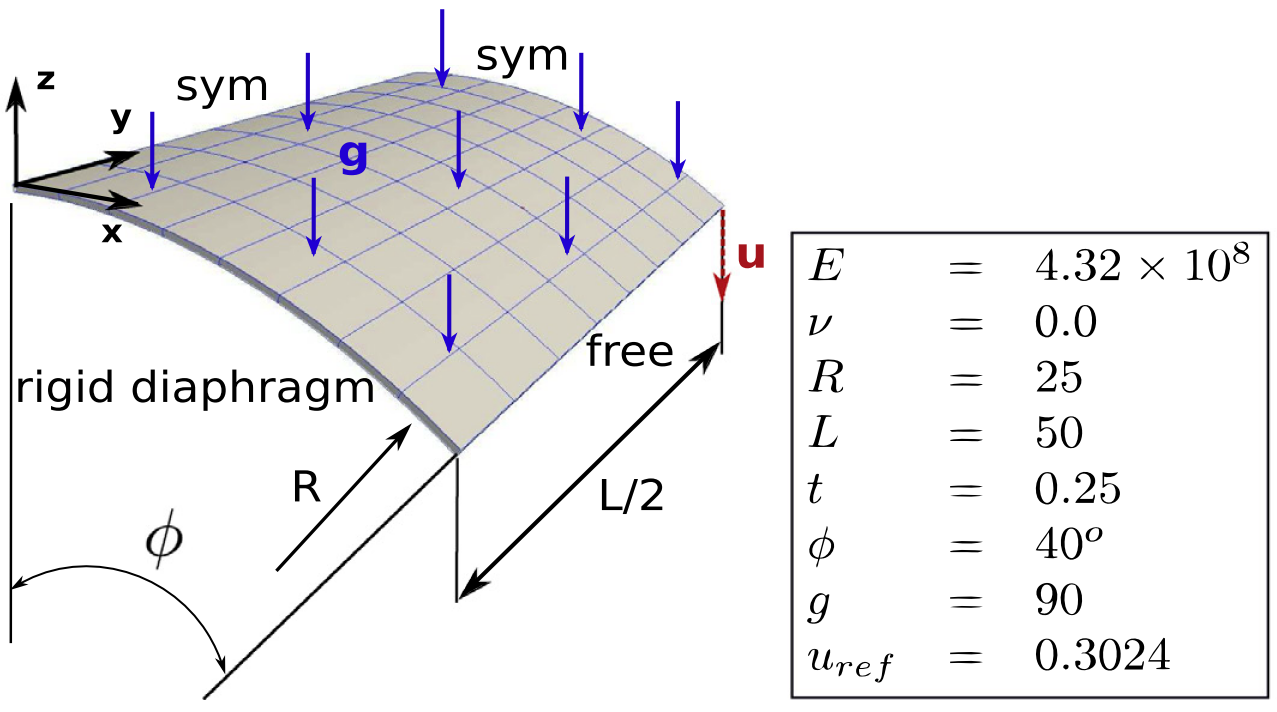
\includegraphics[width=0.40\textwidth]{images/scordelisroof.png}
%	\caption{Definition of the Scordelis-Lo roof benchmark\cite{Bou13}}
%\end{wrapfigure}

The first problem of the shell obstacle course is the Scordelis-Lo roof, which is part of a cylindrical shell fixed by rigid diaphragms at it's axial ends. The loading is a pseudo-gravity distributed load that has a magnitude of 90. Due to symmetry, only a quarter of the shell is modelled. The key result is the vertical displacement of the lateral side at the midpoint, denoted by $\textcolor{red}{u}$ in the following diagram. The reference value is $u_{ref} = 0.3024$.
 
  \begin{figure}[H]
 	\centering
 	\def\svgwidth{\columnwidth}
 	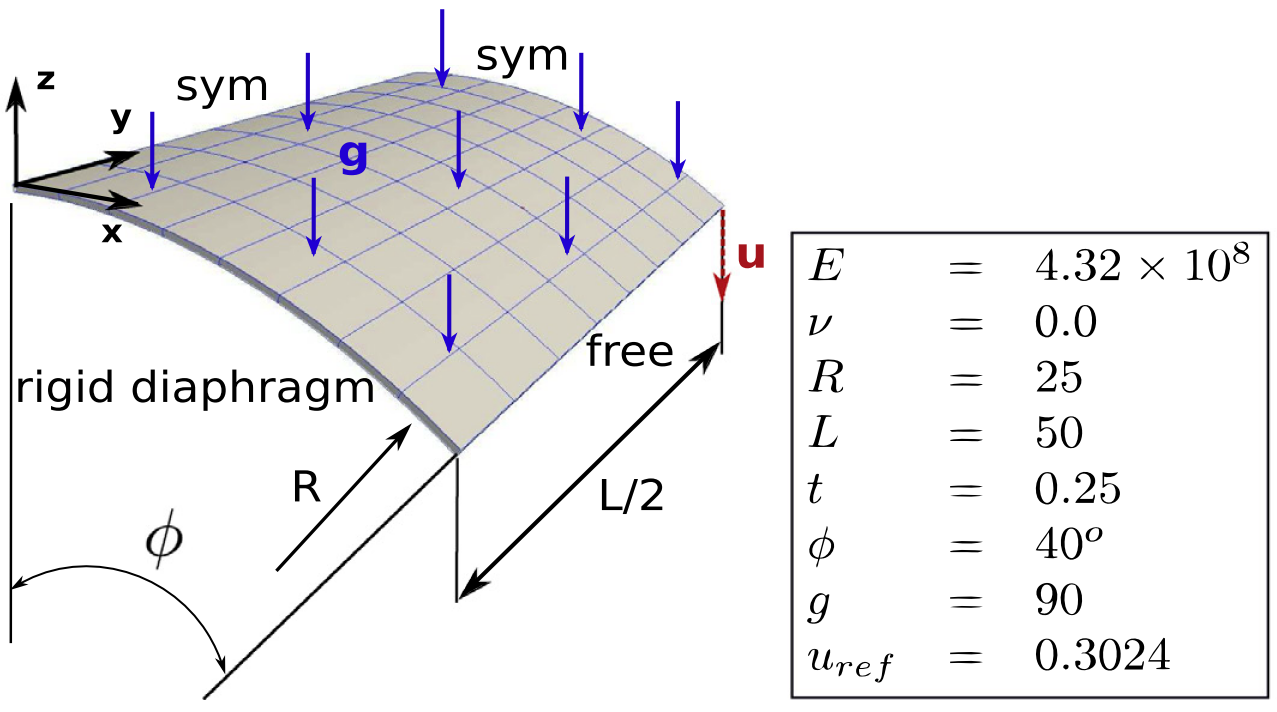
\includegraphics[width=7.3cm]{images/scordelisroof.png}
 	\caption{Definition of the Scordelis-Lo roof benchmark\cite{Bou13}}
 \end{figure}
 
\begin{figure}[H]
	\subfloat[Quadrilateral element convergence for the Scordelis-Lo roof benchmark]
	{\label{ref_label2}
		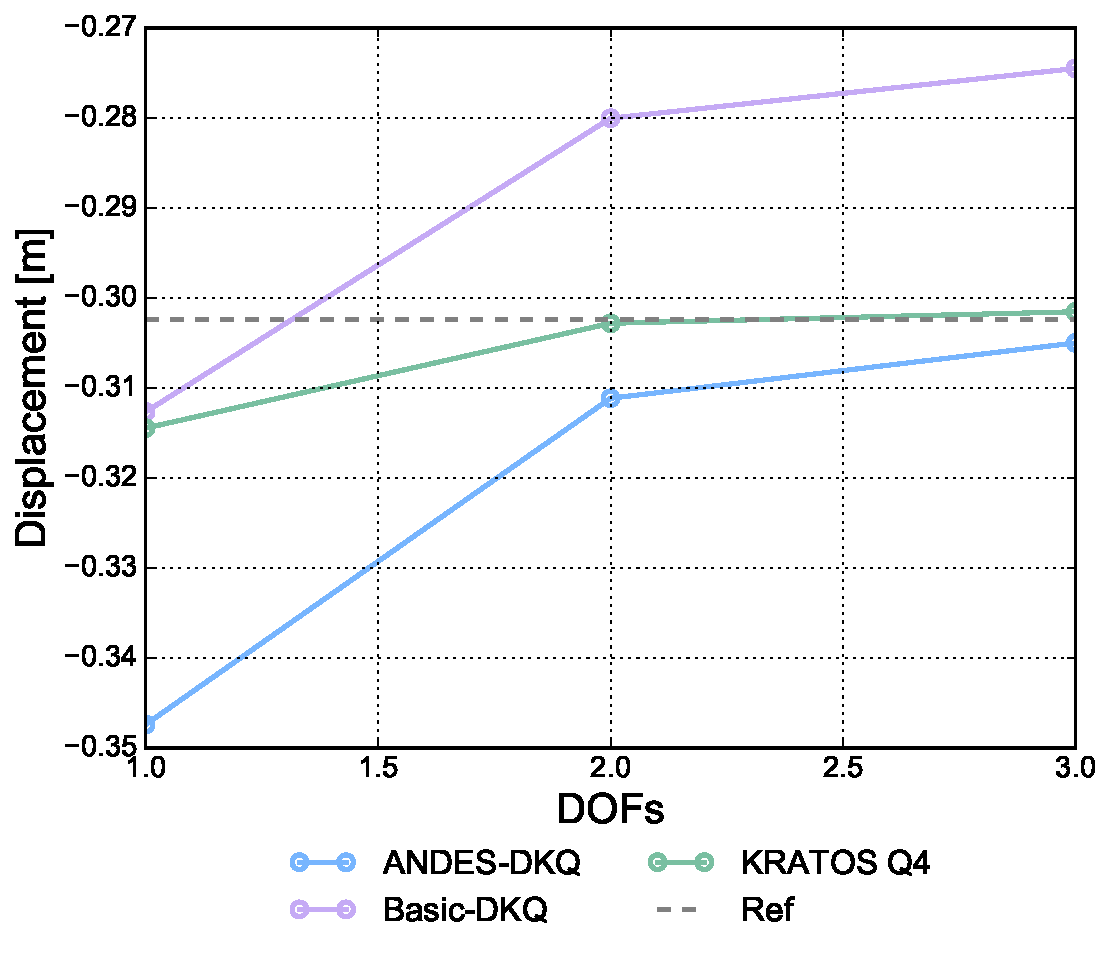
\includegraphics[width=7.3cm]
		{scordelis_structured_quad_results.pdf}}
	\subfloat[Triangle element convergence for the Scordelis-Lo roof benchmark]
	{\label{ref_label2}
		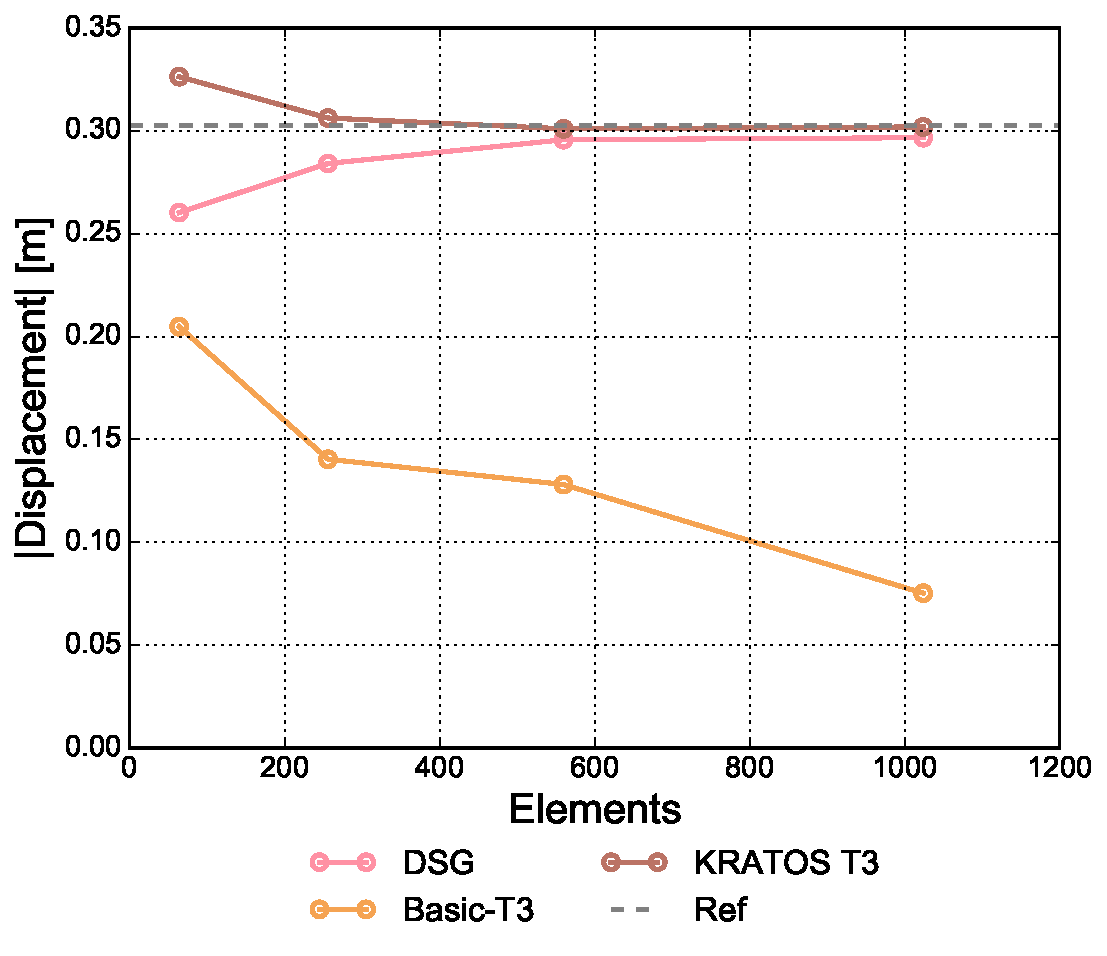
\includegraphics[width=7.3cm]
		{scordelis_structured_tri_results.pdf}}
	\caption{\label{ref_label_overall}Scordelis-Lo roof benchmark results}
\end{figure}

The convergence graphs above indicate the ANDES-DKQ and DSG elements agree to the reference solution. Conversely, the Basic-T3 element shows very poor performance. Given that the Basic-DKQ performs well (which is immune to transverse shear locking), it's suspected that transverse shear locking is crippling the Basic-T3 element, while the DSG element technology effectively mitigates this for the DSG element. 
\newpage
\subsection{Pinched cylinder - good}
%
%\begin{wrapfigure}{r}{0.45\textwidth}
%	\centering
%	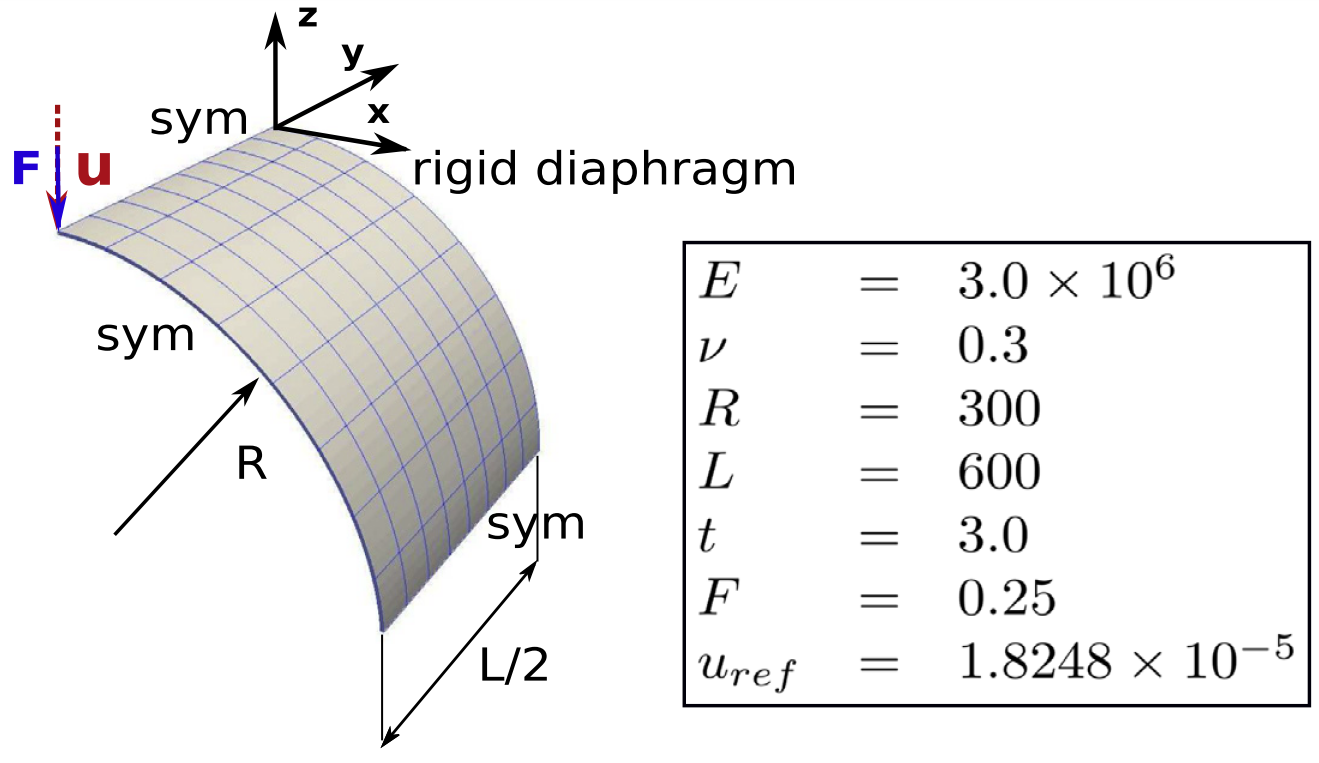
\includegraphics[width=0.4\textwidth]{images/pinchedcylinder.png}
%	\caption{Definition of the pinched cylinder benchmark\cite{Bou13}}
%\end{wrapfigure}

The second problem of the shell obstacle course is the pinched cylinder, which considers a cylindrical shell fixed by rigid diaphragms at it's axial ends. The loading consists of two opposing compressive point loads at the centre of the shell. Due to symmetry only an eighth of the shell is modelled. The key result is the vertical displacement under the point load, denoted by $\textcolor{red}{u}$ in the following diagram. The reference value is $u_{ref} =  1.8248\ \times\ 10^{-5}$. 
 
 \begin{figure}[H]
 	\centering
 	\def\svgwidth{\columnwidth}
 	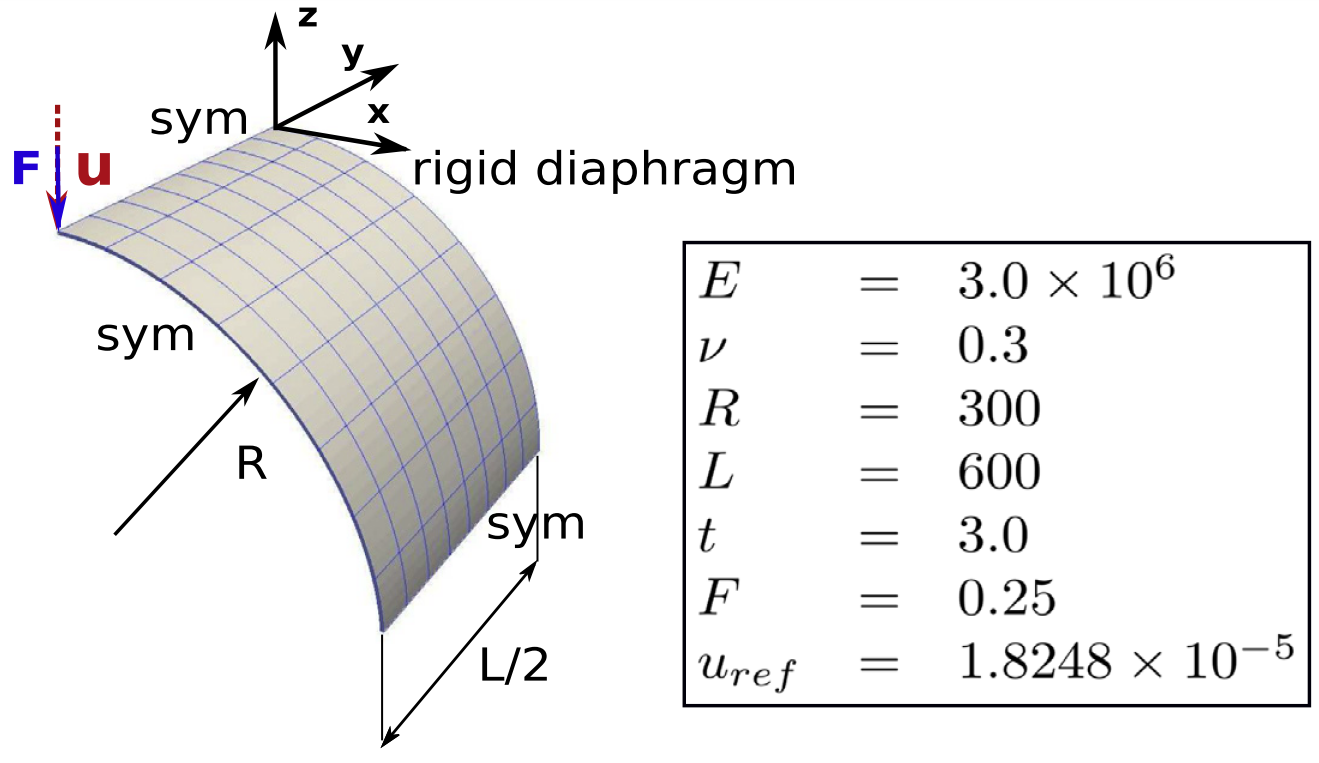
\includegraphics[width=7.3cm]{images/pinchedcylinder.png}
 	\caption{Definition of the pinched cylinder benchmark\cite{Bou13}}
 \end{figure}
 
\begin{figure}[H]
	\subfloat[Quadrilateral element convergence for the pinched cylinder benchmark]
	{\label{ref_label2}
		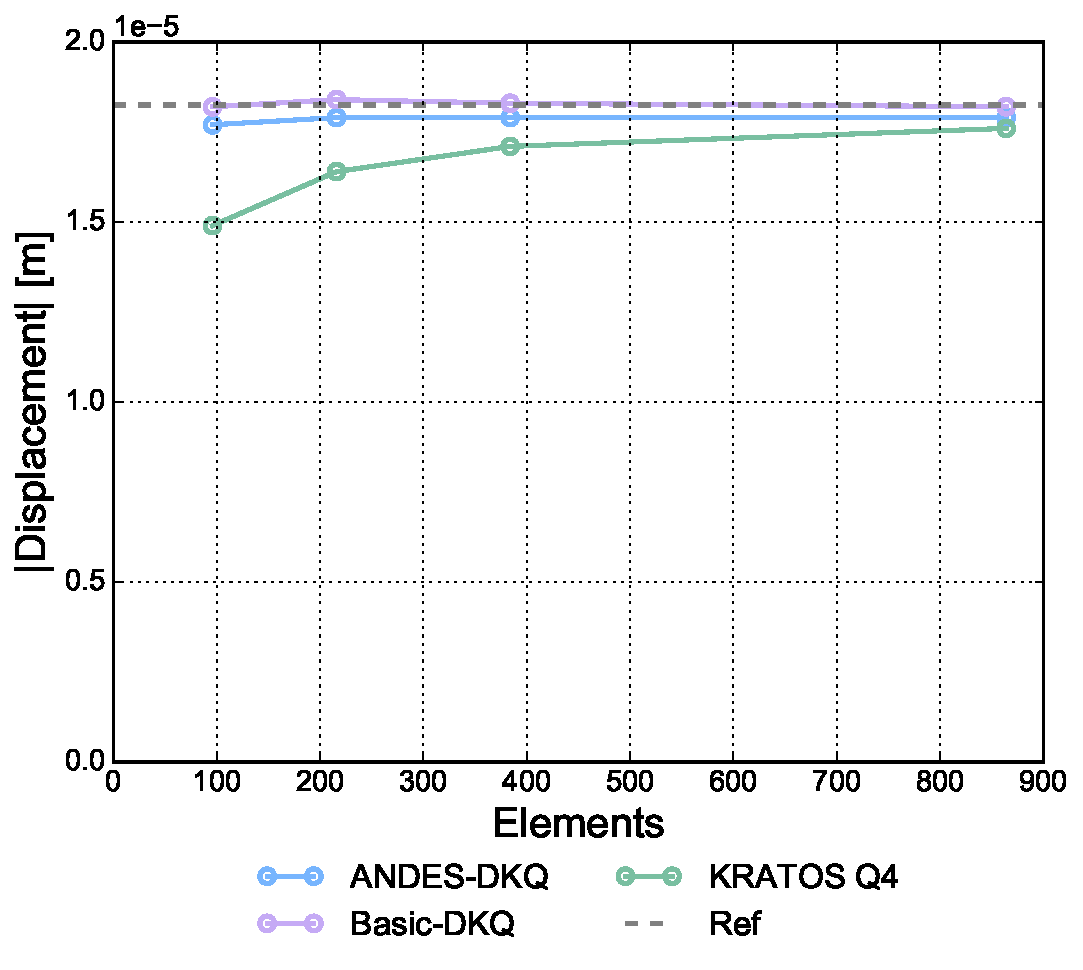
\includegraphics[width=7.3cm]
		{pinched_cyl_structured_quad_results.pdf}}
	\subfloat[Triangle element convergence for the pinched cylinder benchmark]
	{\label{ref_label2}
		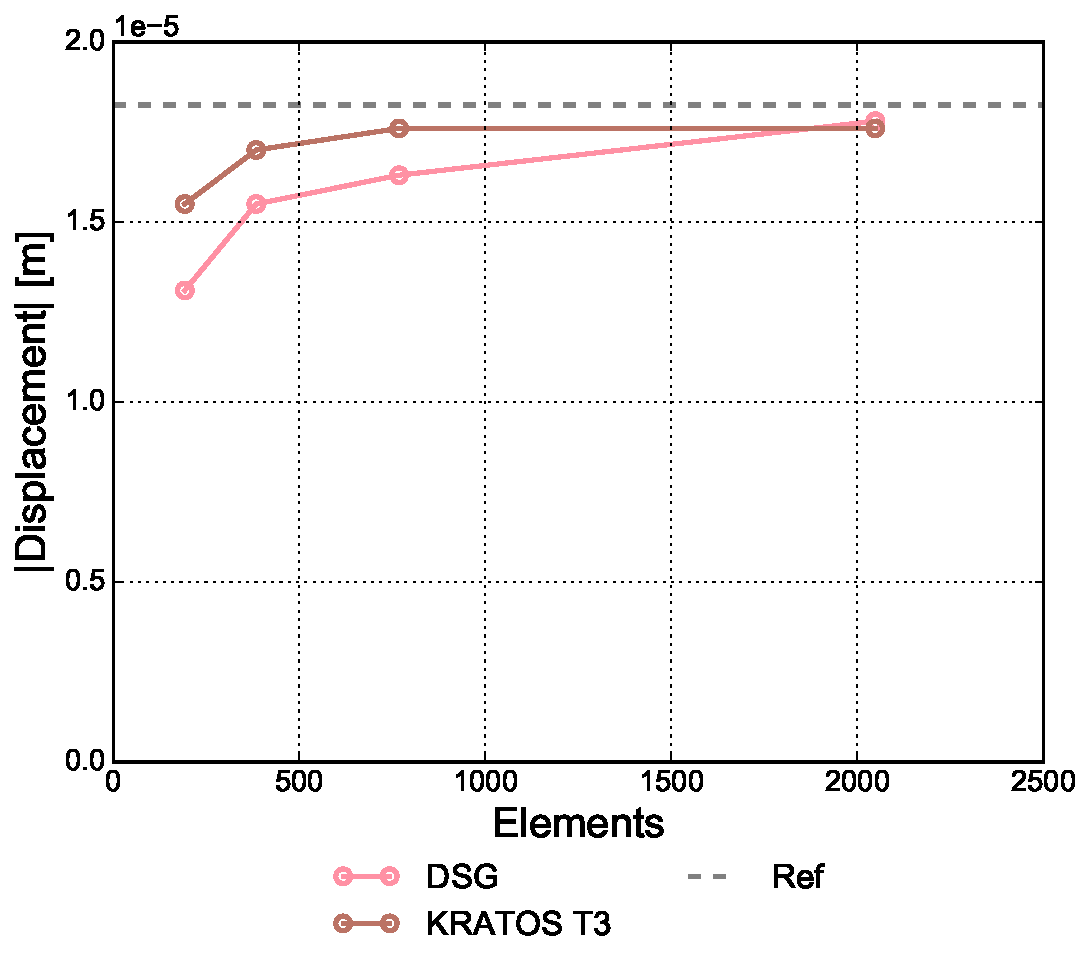
\includegraphics[width=7.3cm]
		{pinched_cyl_structured_tri_results.pdf}}
	\caption{\label{ref_label_overall}Pinched cylinder benchmark results}
\end{figure}

 The good performance of both the ANDES-DKQ and DSG elements is demonstrated in the convergence graphs above. The Basic-T3 results were in the order of $1\times10^{-3}$ (roughly 100 times greater than the reference solution) and were omitted from the graph for clarity of scale. Once again, it is clear that the computationally inexpensive DSG element technology drastically improves performance from the un-enhanced Basic-T3 to the DSG element.
\newpage
\subsection{Pinched hemisphere - good}
%
%\begin{wrapfigure}{r}{0.45\textwidth}
%	\centering
%	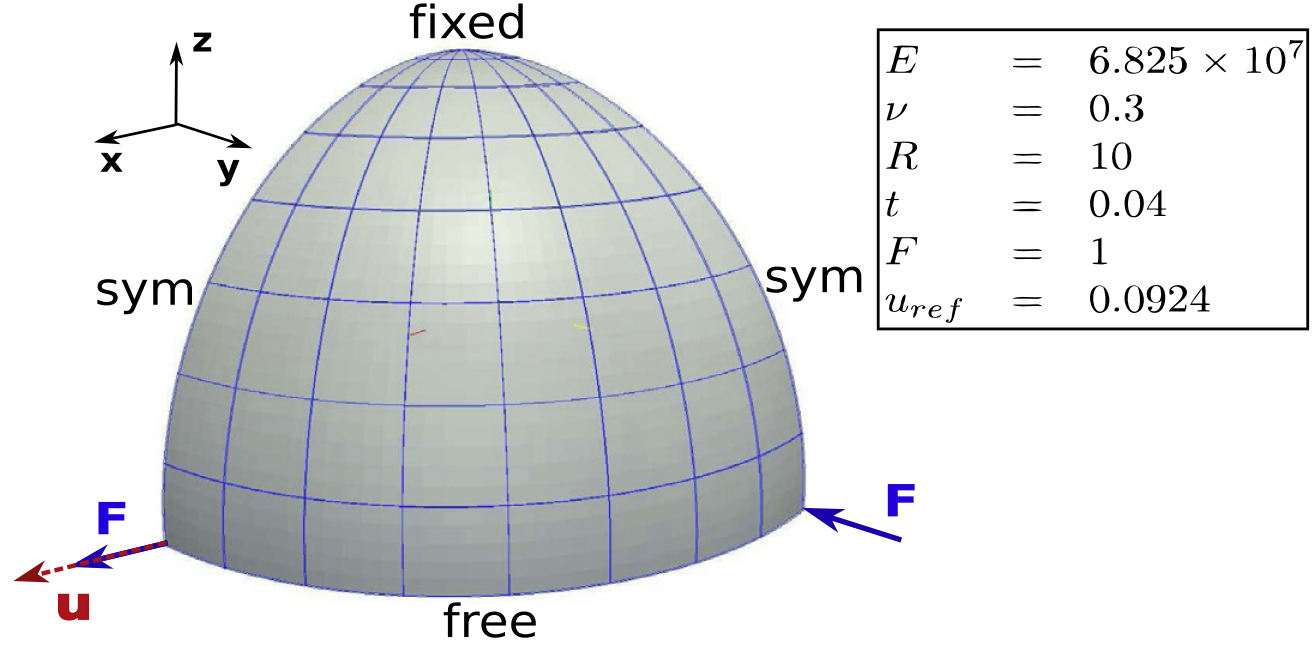
\includegraphics[width=0.4\textwidth]{images/pinchedhemisphere.png}
%	\caption{Definition of the pinched hemisphere benchmark \cite{Bou13}}
%\end{wrapfigure}

The last test in the shell obstacle course is the pinched hemisphere, which considers a hemispherical shell loaded with opposing point loads along it's equator. Due to symmetry only a quarter of the shell is modelled. The key result is the 'x' displacement along one of the point loads, denoted by $\textcolor{red}{u}$ in the following diagram. The reference value is $u_{ref} =  0.0924$. 

\begin{figure}[H]
	\centering
	\def\svgwidth{\columnwidth}
	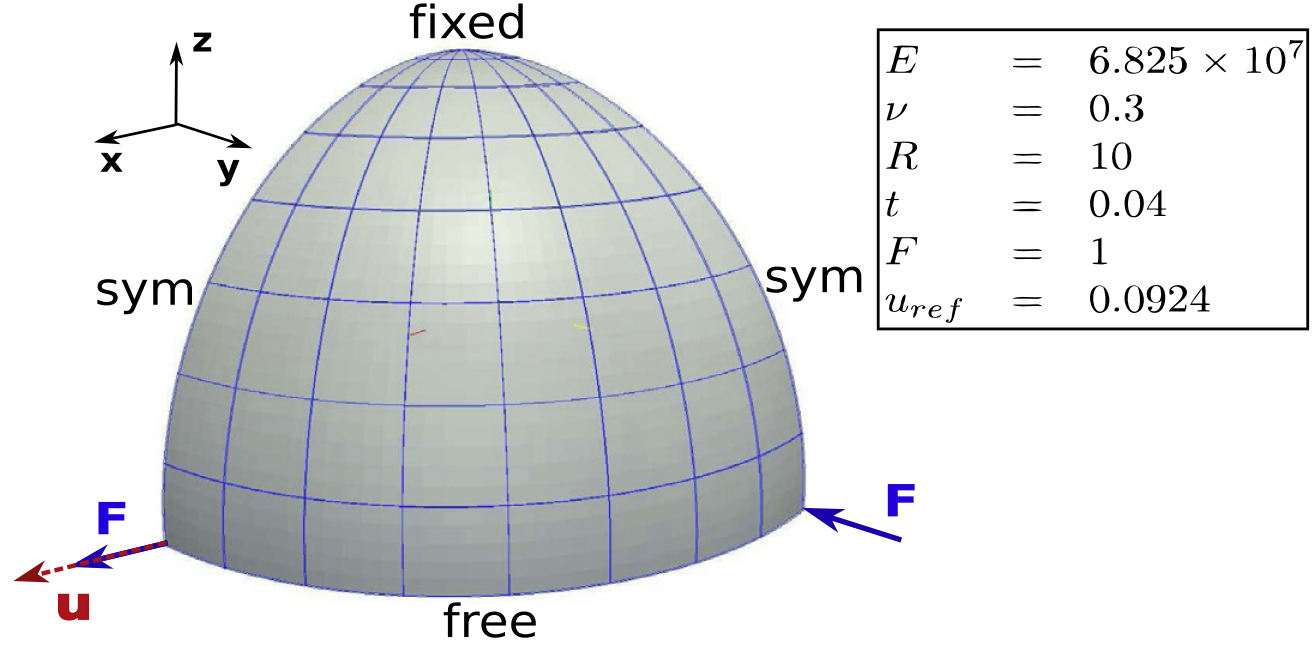
\includegraphics[width=7.3cm]{images/pinchedhemisphere.png}
	\caption{Definition of the pinched hemisphere benchmark \cite{Bou13}}
\end{figure}

\begin{figure}[H]
	\subfloat[Quadrilateral element convergence for the pinched hemisphere benchmark]
	{\label{ref_label2}
		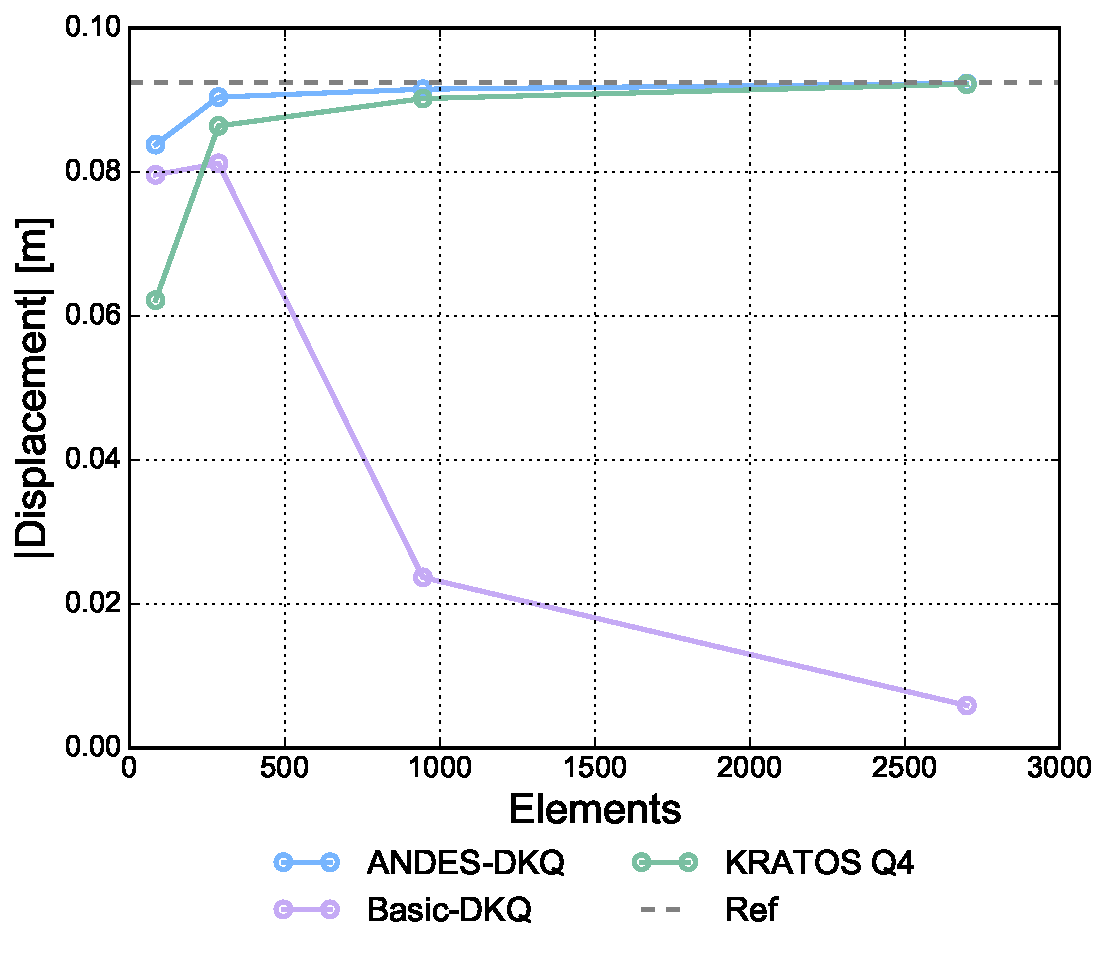
\includegraphics[width=7.3cm]
		{pinched_hemi_quad_results.pdf}}
	\subfloat[Triangle element convergence for the pinched hemisphere benchmark]
	{\label{ref_label2}
		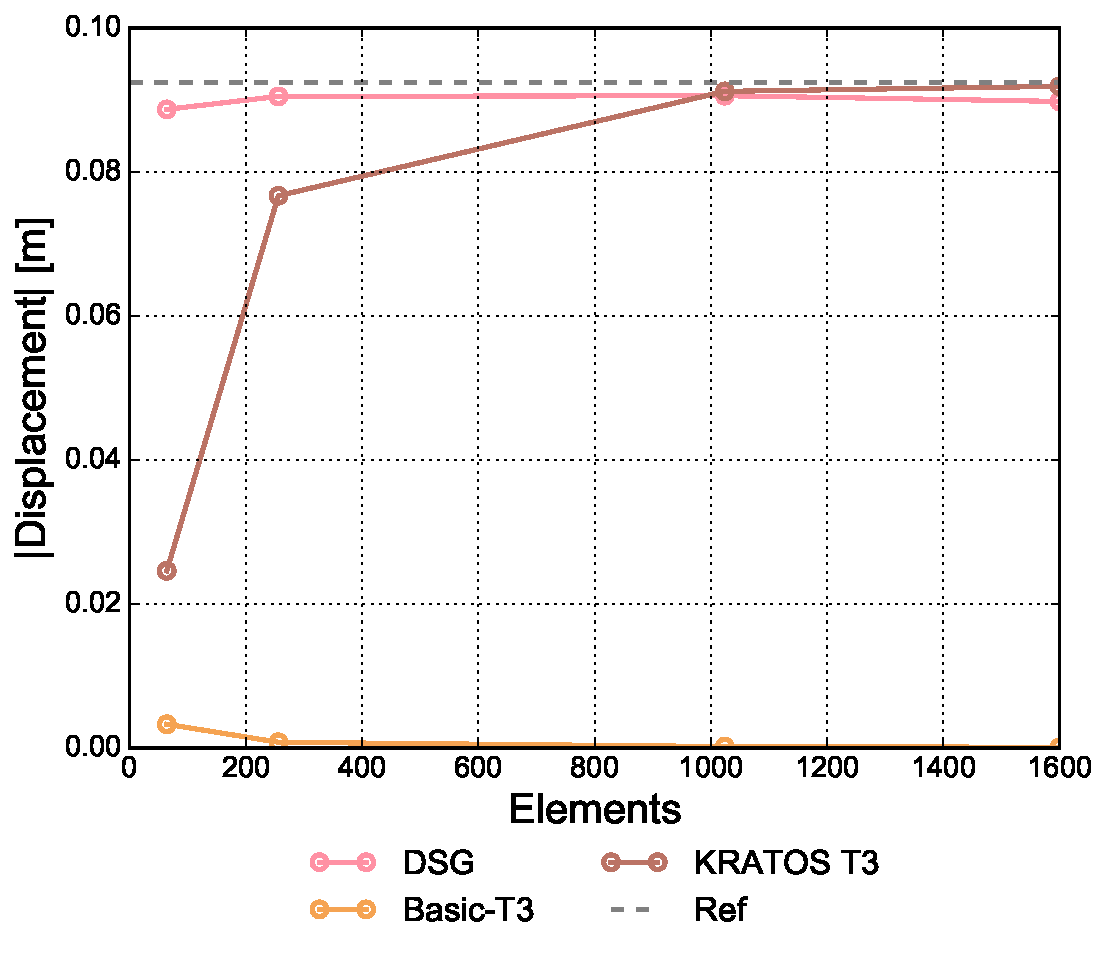
\includegraphics[width=7.3cm]
		{pinched_hemi_tri_results.pdf}}
	\caption{\label{ref_label_overall}Pinched hemisphere benchmark results}
\end{figure}

The ANDES-DKQ and DSG elements both perform well in the final statics test, as per the convergence graphs above. It is observed that the Basic-DKQ element appears to exhibit membrane locking corresponding to the high double curvature of the problem ($R_1=R_2 = 10$) compared to the Scordelis-Lo roof ($R_1= 10,\ R_2 = \infty$) and the pinched cylinder ($R_1= 300,\ R_2 = \infty$). The ANDES element technology clearly prevents this deleterious effect. The poor performance of the Basic-T3 element compared to the DSG element once again highlights the effectiveness of the DSG element technology in preventing transverse shear locking.
\newpage
\section{Geometically non-linear benchmarks}

Large rotations and displacements mark the departure from geometrically linear to non-linear analyses, however, the assumption of small strains is still maintained. The extension of the elements to geometrically non-linear problems is handled by employing an existing Kratos class which provides co-rotational transformations for shells. At each increment in the non-linear solution, the large displacements and rotations of each element is mapped by rigid body translations and rotations, thus limiting the strains experienced by the element to reasonably small magnitudes. The performance of the element in geometrically non-linear problems is considered with two benchmarks.

\subsection{Hinged cylindrical roof - good}

The first geometrically non-linear benchmark is the snap-through of a hinged cylindrical roof under a central point load $P_{max} = 3000$ \cite{Sze2004}. As per the diagram below, the roof geometry is defined with the parameters: $L = 254,\ R = 2540,\ \theta=0.1\ rad$ and $t = 12.7$. The material is defined with a Young's modulus $E = 3102.75$ and Poisson's ratio of $\nu = 0.3$.

 
\begin{figure}[H]
	%\centering
	\subfloat[Hinged cylindrical roof definition \cite{Sze2004}]
	{\label{ref_label1}
		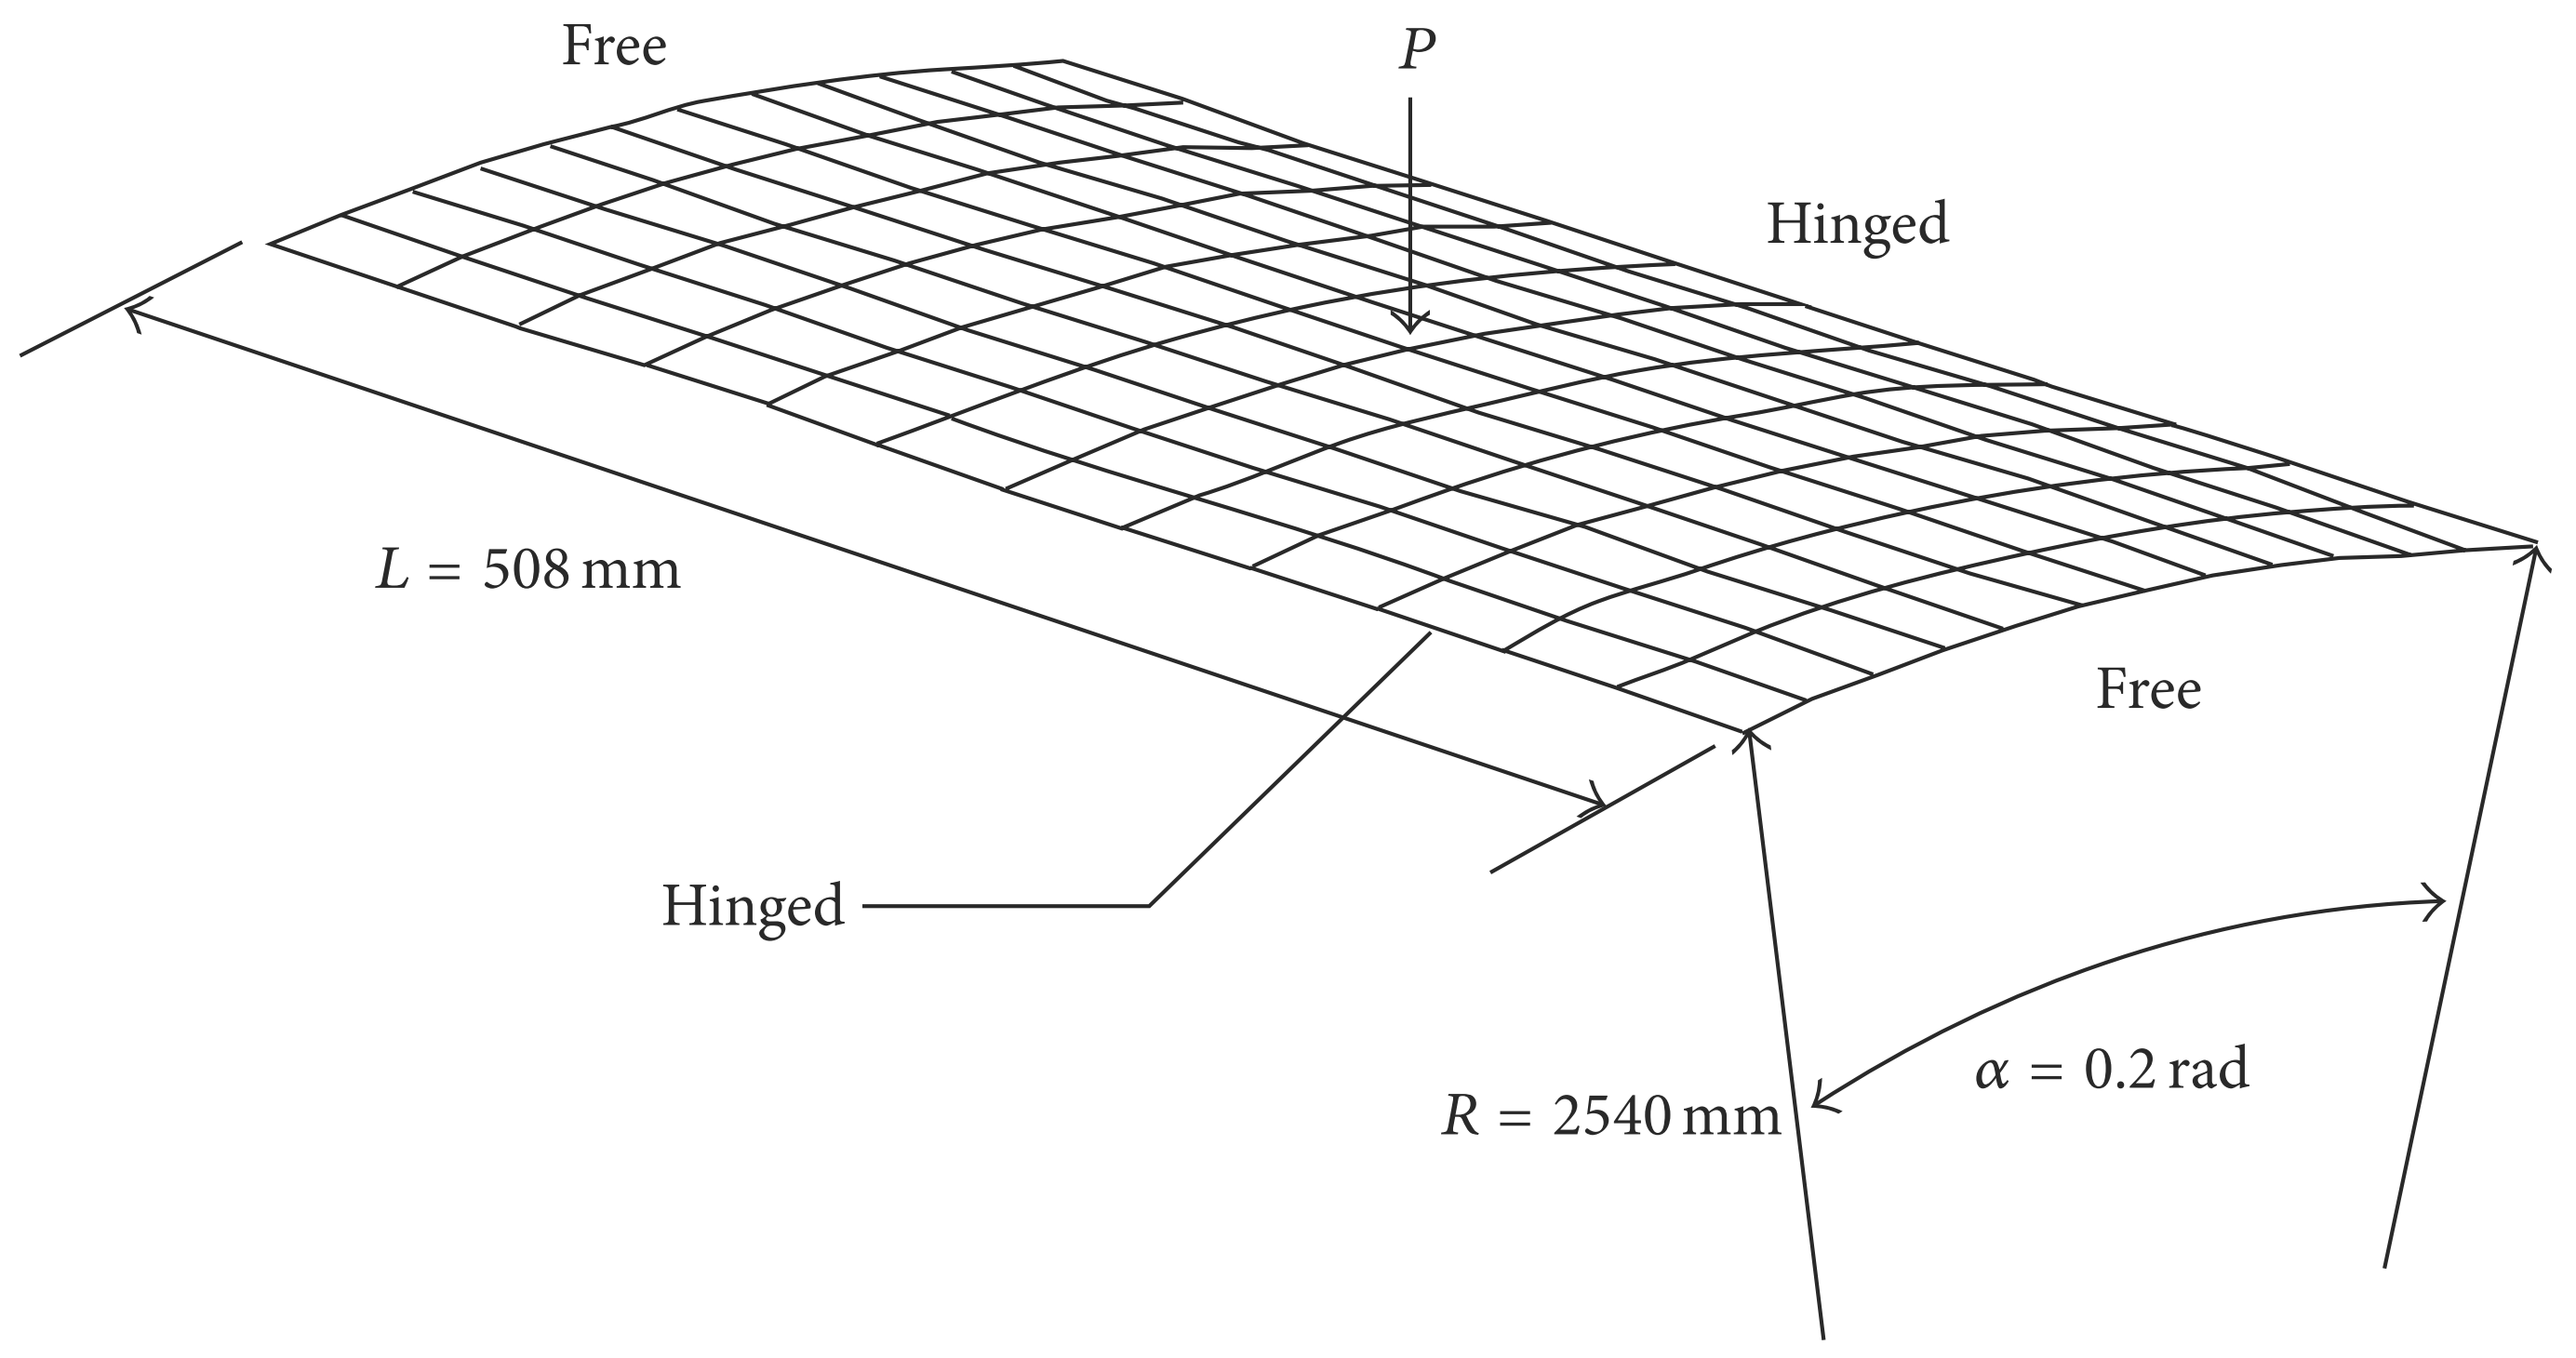
\includegraphics[width=7.3cm]
		{images/hinged_cylindrical_roof.png}}
	\subfloat[Load-displacement curve of hinged cylindrical roof]
	{\label{ref_label2}
		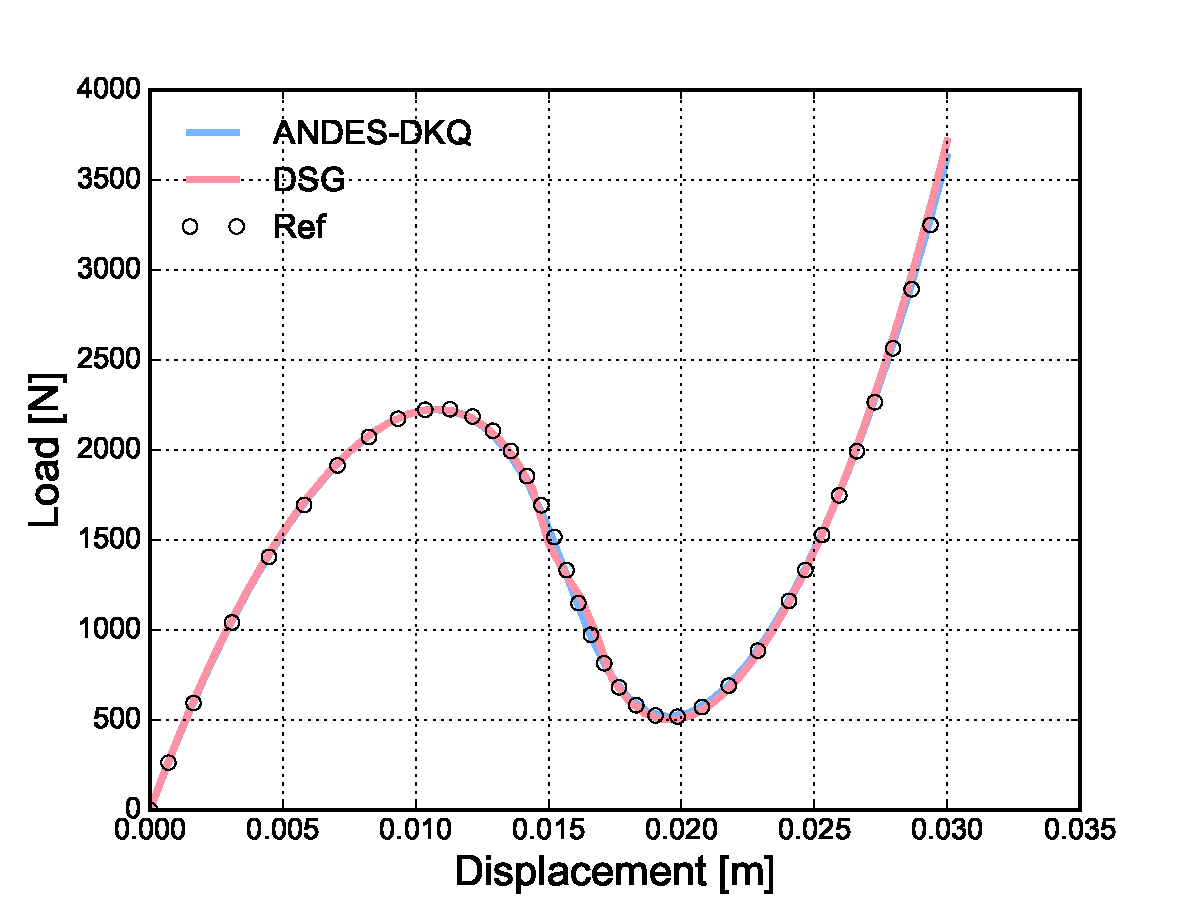
\includegraphics[width=7.3cm]
		{Load_displacement_curve_hinged_cylindrical_roof.pdf}}
	\caption{\label{ref_label_overall}Hinged cylindrical roof benchmark}
\end{figure}

 
The load displacement curve plots the equilibrium path for the ANDES-DKQ and DSG elements against the reference path from \cite{Sze2004}. The full equilibrium path isn't resolved because Kratos only has a load control non-linear solution method implemented, translating to the restriction of only resolving monotonically increasing paths. Regardless, both elements clearly follow the initial path, and then rejoin the reference solution to correctly resolve the structure in it's snapped-through state.

\newpage
\subsection{Open cylinder pull-out - good}

The second geometrically non-linear benchmark is the pull-out of an open cylinder with a load $P_{max} = 40\ 000$. The geometry of the cylinder is $L= 10.35,\ R = 4.953$ and $t = 0.094$ while the linear elastic material is characterised by $E = 10.5\times10^6$ and $\nu = 0.3125$. The measured displacement is the vertical deformation $u_z$ at the point of load application.

 
\begin{figure}[H]
	%\centering
	\subfloat[Open cylinder pullout definition \cite{Sze2004}]
	{\label{ref_label1}
		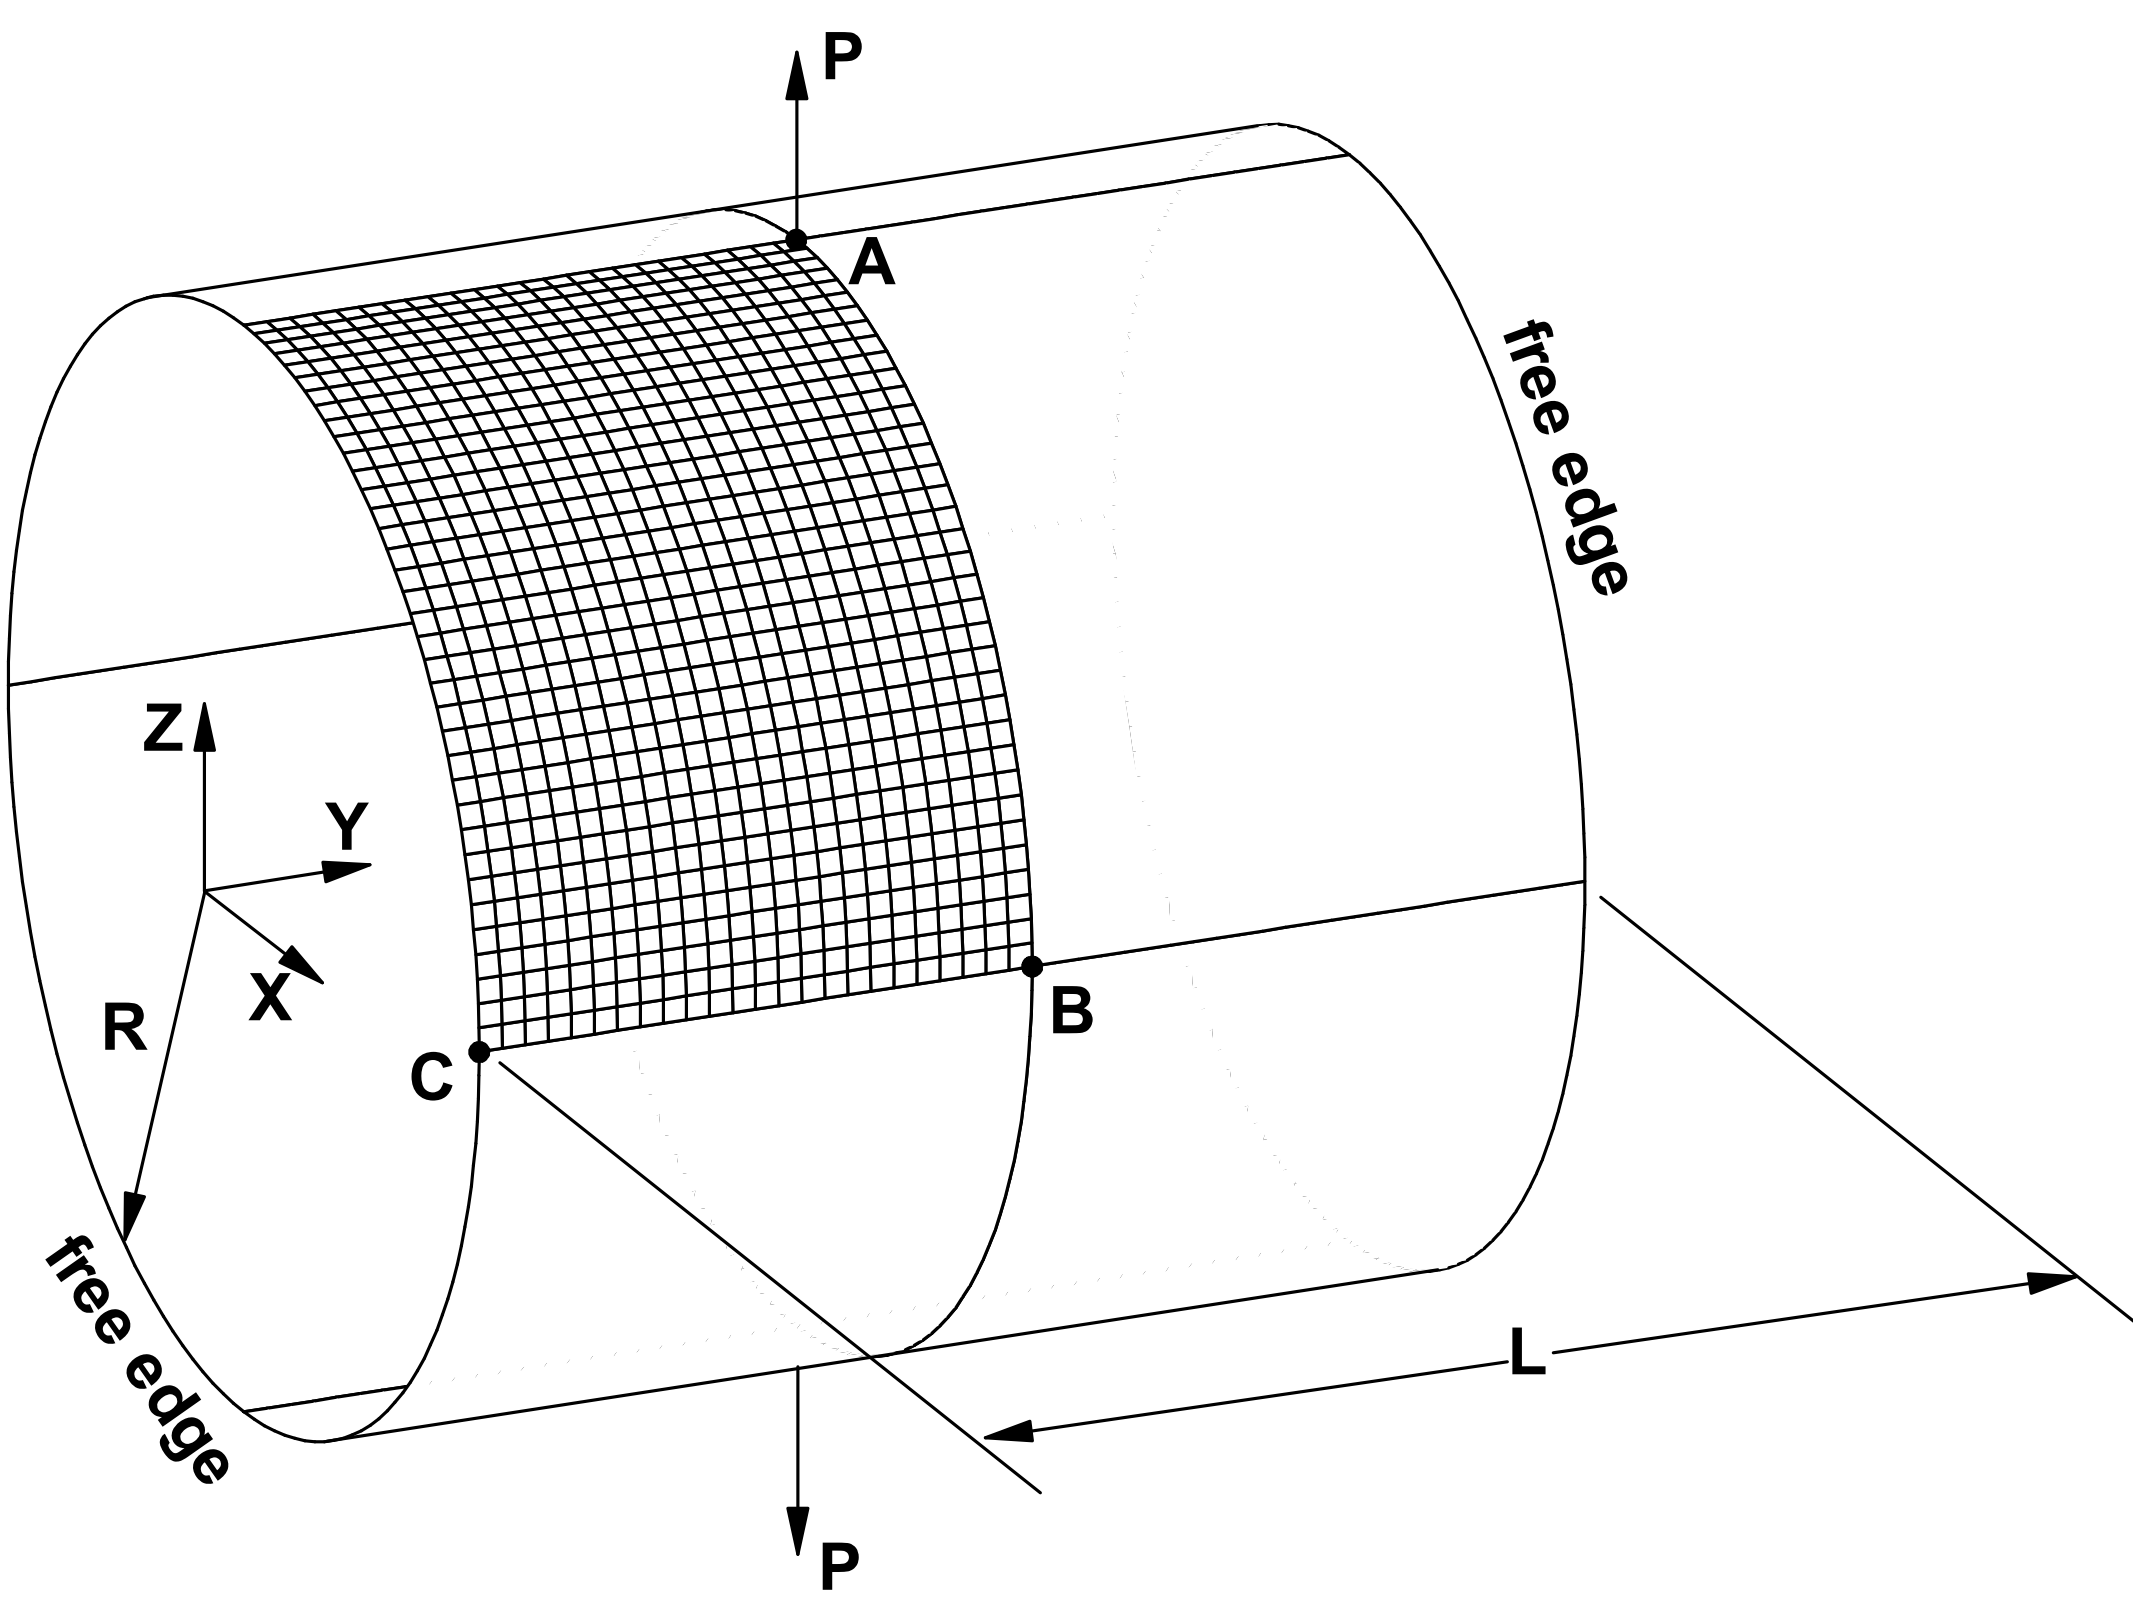
\includegraphics[width=7.3cm]
		{images/opencylinderpullout.png}}
	\subfloat[Load-displacement curve of open cylinder pullout]
	{\label{ref_label2}
		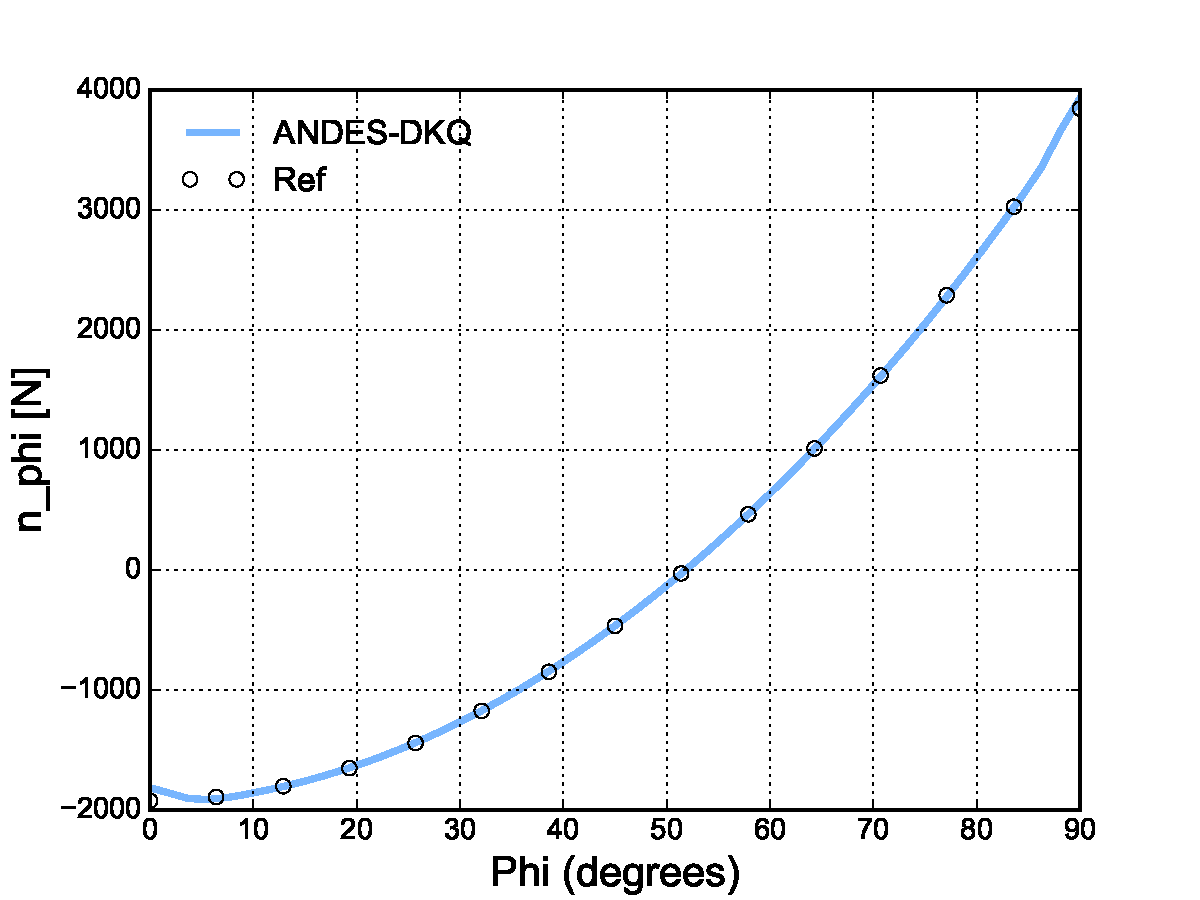
\includegraphics[width=7.3cm]
		{Load_displacement_curve_open_cylinder_pullout.pdf}}
	\caption{\label{ref_label_overall}Open cylinder pullout benchmark}
\end{figure}

 The load-displacement curve above plots the equilibrium path for the ANDES-DKQ and DSG elements against the reference solution \cite{Sze2004}. Although both elements closely follow the reference path, the ANDES-DKQ performs better in this test than the DSG element. Despite this, the error of the DSG element at maximum load is still only 1.7\%.

\section{Dynamics benchmarks}

Dynamic problems introduce inertial effects into the array of phenomena analysed. Combined with the aforementioned co-rotational formulation, it is possible to accurately resolve bodies undergoing large movements over time.

\subsection{Shell pendulum - good}

The first dynamic benchmark is a simple shell pendulum allowed to freely rotate along one hinged edge. The initial horizontal configuration of the $1m\times1m\times0.1m$ thick square plate is subject to gravity $g = 9.8\ m/s^2$ acting in the vertical $Z$ direction. The material of the plate is described by $E = 1\times 10^9 Pa,\ \nu = 0.0$ and $\rho = 7850 kg/m^3$. The key result is the vertical displacement component of the free corner node as drawn below.
 
\begin{figure}[H]
	%\centering
	\subfloat[Shell pendulum definition]
	{\label{ref_label1}
		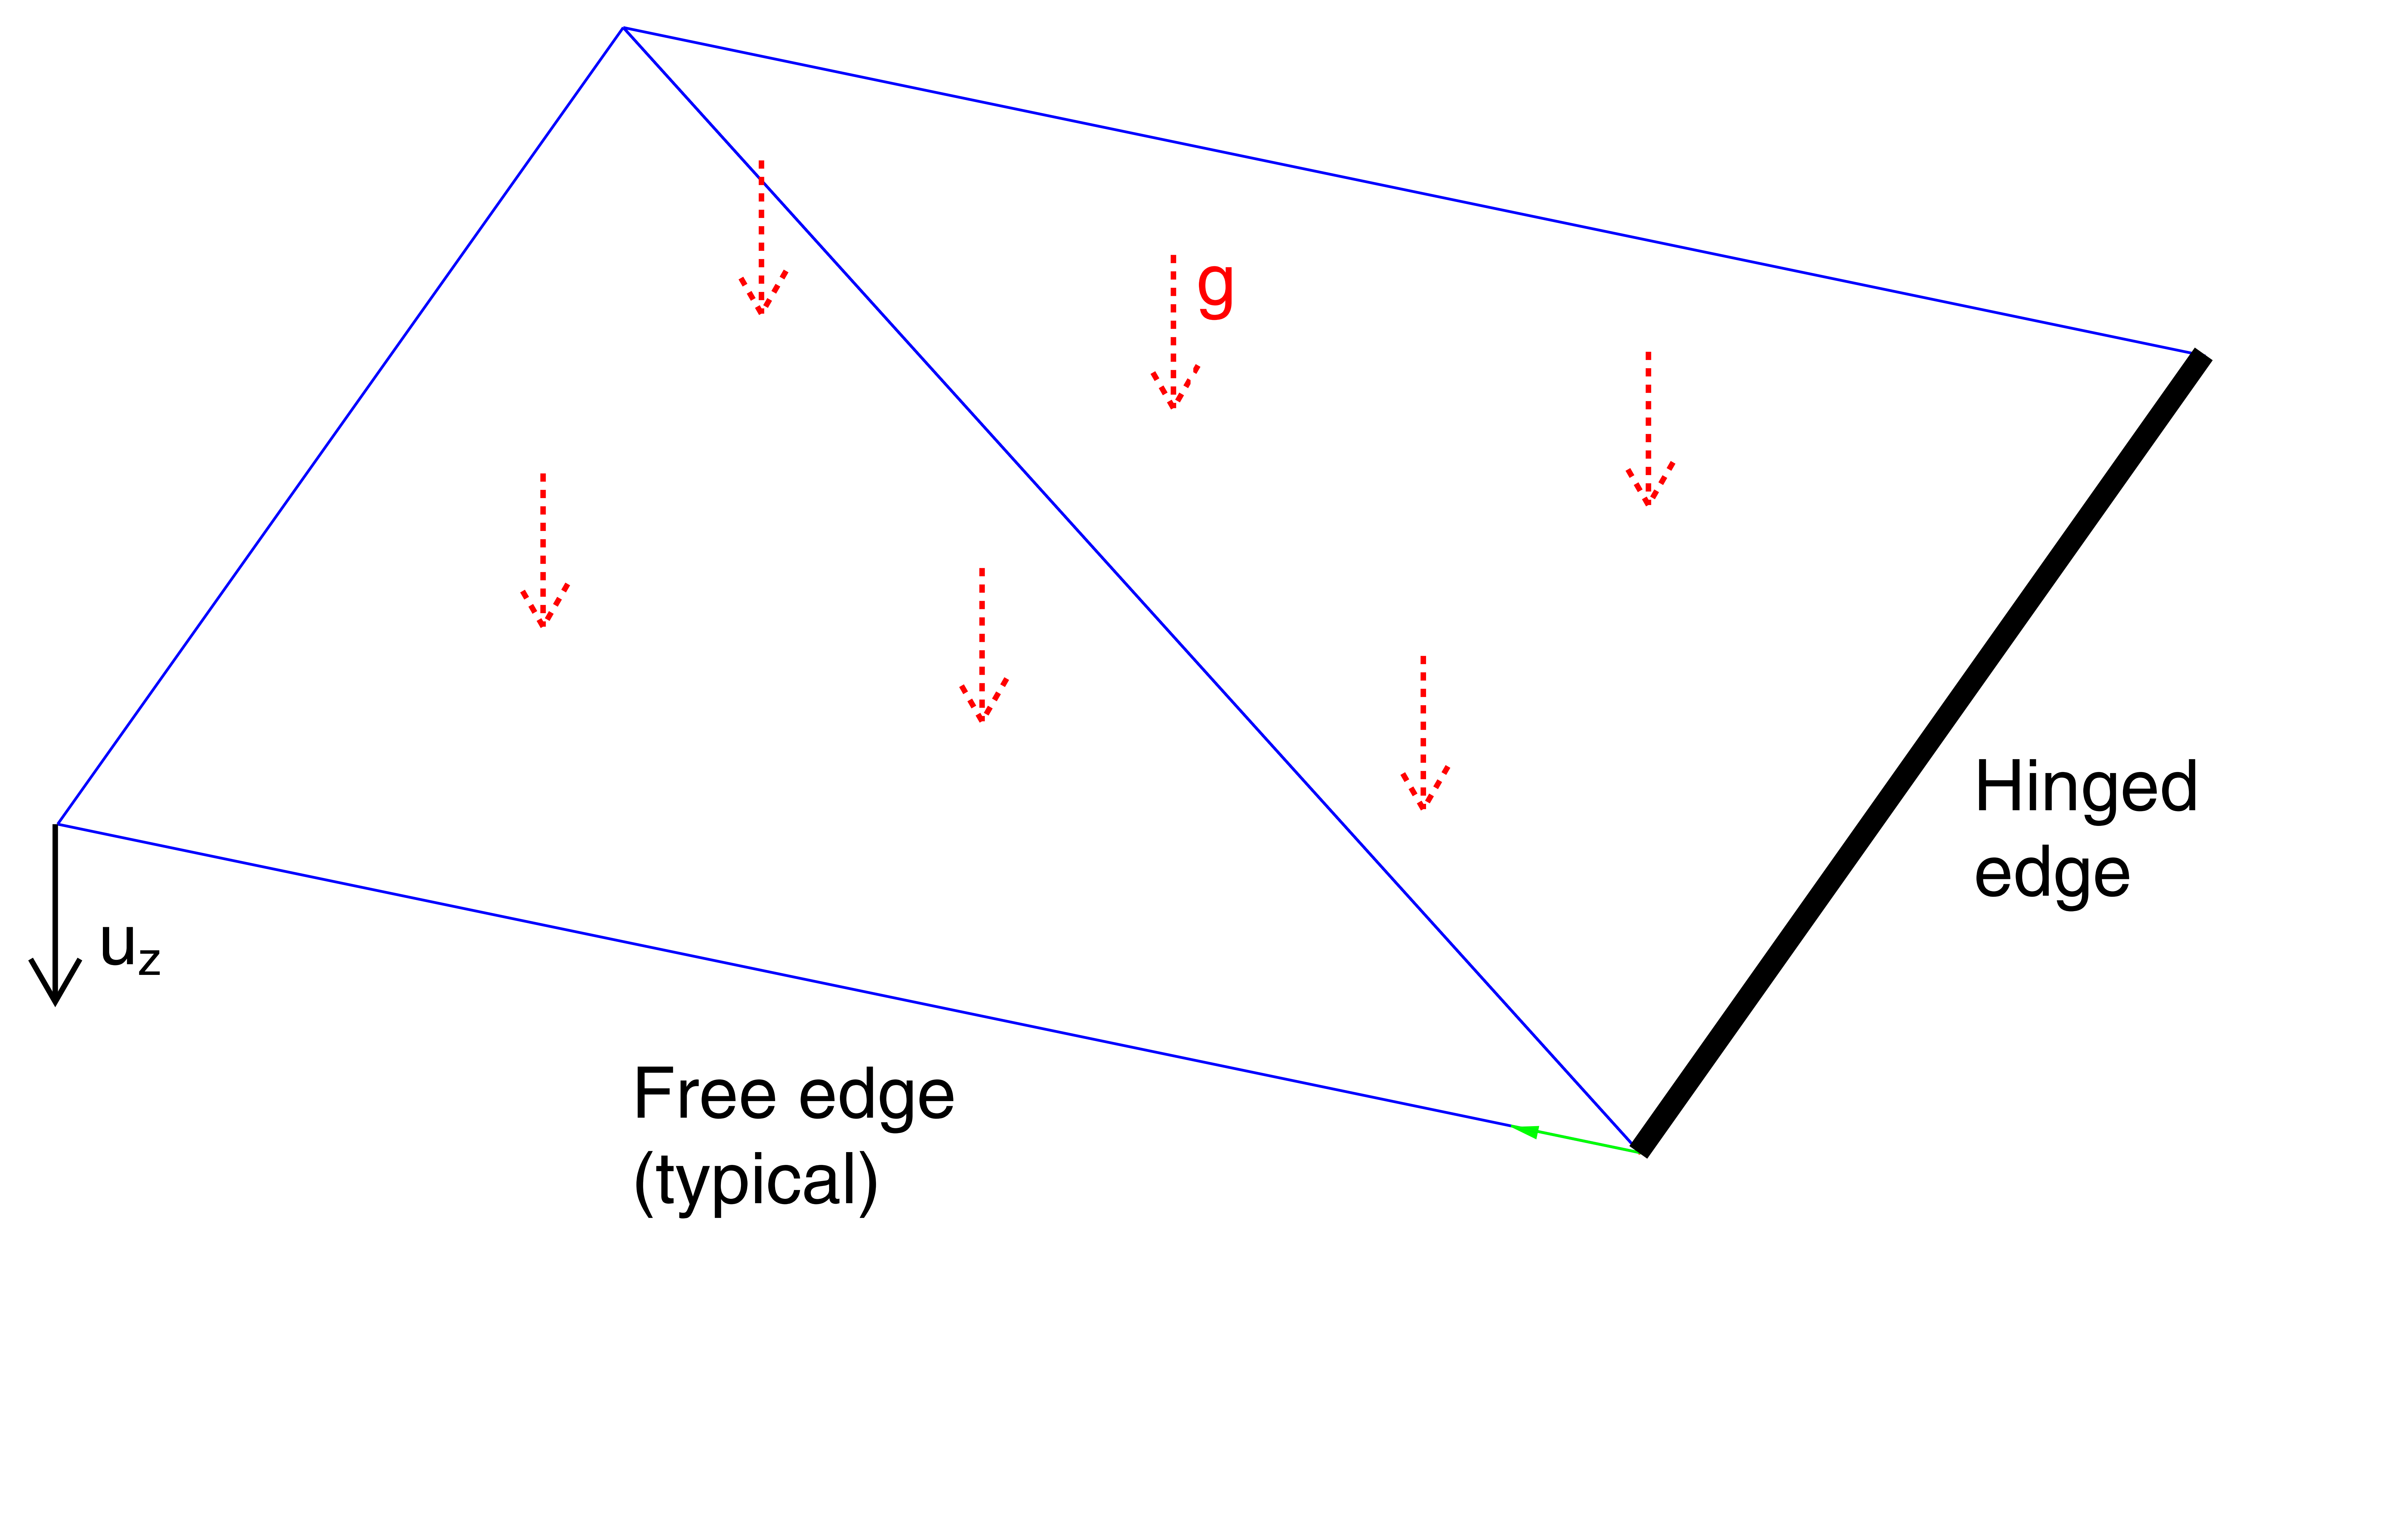
\includegraphics[width=7.3cm]
		{images/swinging_plate_problem.png}}
	\subfloat[Vertical displacement over time for shell pendulum benchmark]
	{\label{ref_label2}
		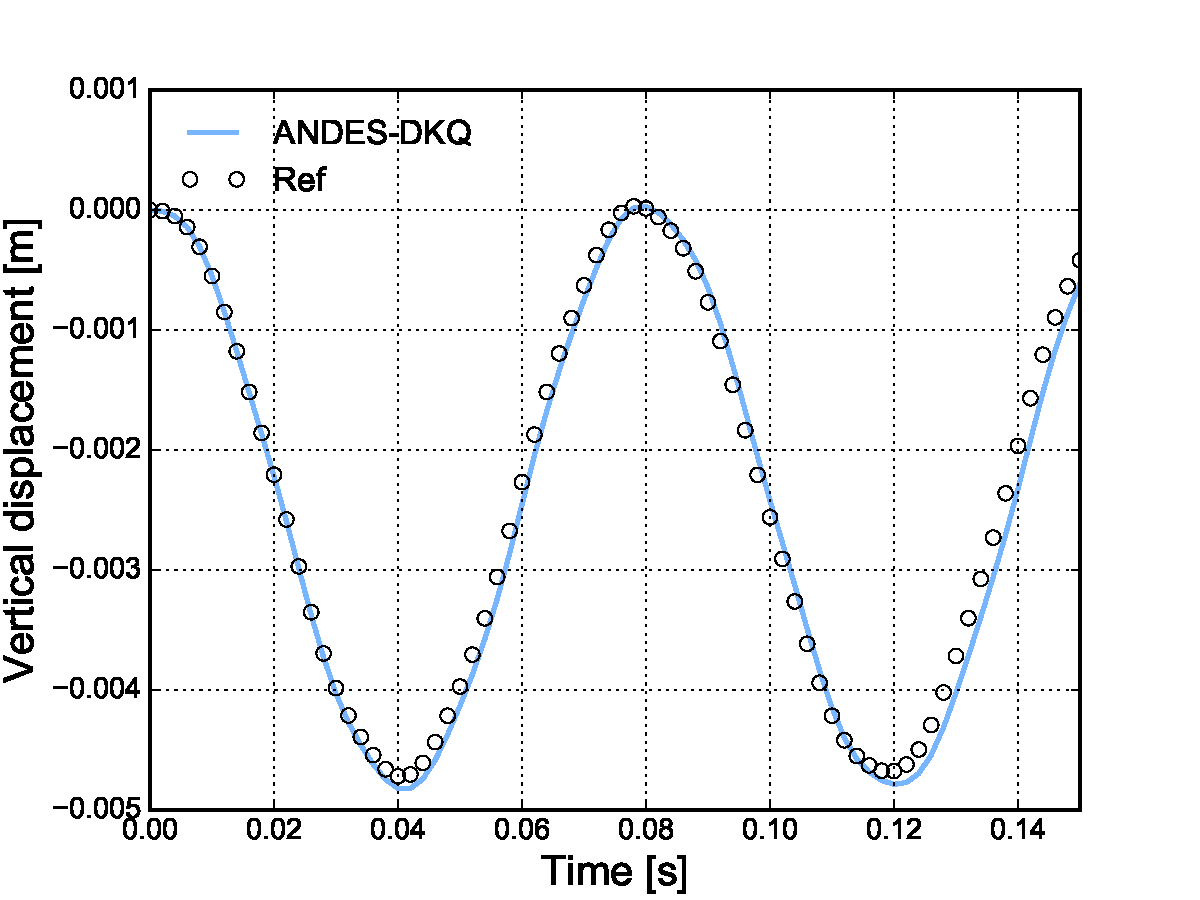
\includegraphics[width=7.3cm]
		{swinging_plate_graph.pdf}}
	\caption{\label{ref_label_overall}Shell pendulum benchmark}
\end{figure}

The plot of displacement over time demonstrates the ability of both elements to handle large displacements and rotations, agreeing with the reference solution of the existing Kratos quadrilateral shell element. As expected, the minimum vertical displacement of $u_z=-1m$ corresponds to the position of bottom dead centre of the plate, while the maximum vertical displacement of $u_z=0m$ corresponds to a fully horizontal plate orientation

\subsection{Oscillating clamped plate - good}

The oscillating clamped plate benchmark subjects a clamped cantilever square plate $2m\times2m\times0.1m$ thick to a uniform globally oriented surface pressure of $P_z = -0.25 Pa$. The plate material is linear elastic characterised by $E = 1\times 10^6 Pa,\ \nu = 0.0$ and $\rho = 7850 kg/m^3$. The key result is the vertical displacement component of the free corner node as illustrated below.
 
\begin{figure}[H]
	%\centering
	\subfloat[Oscillating clamped plate definition]
	{\label{ref_label1}
		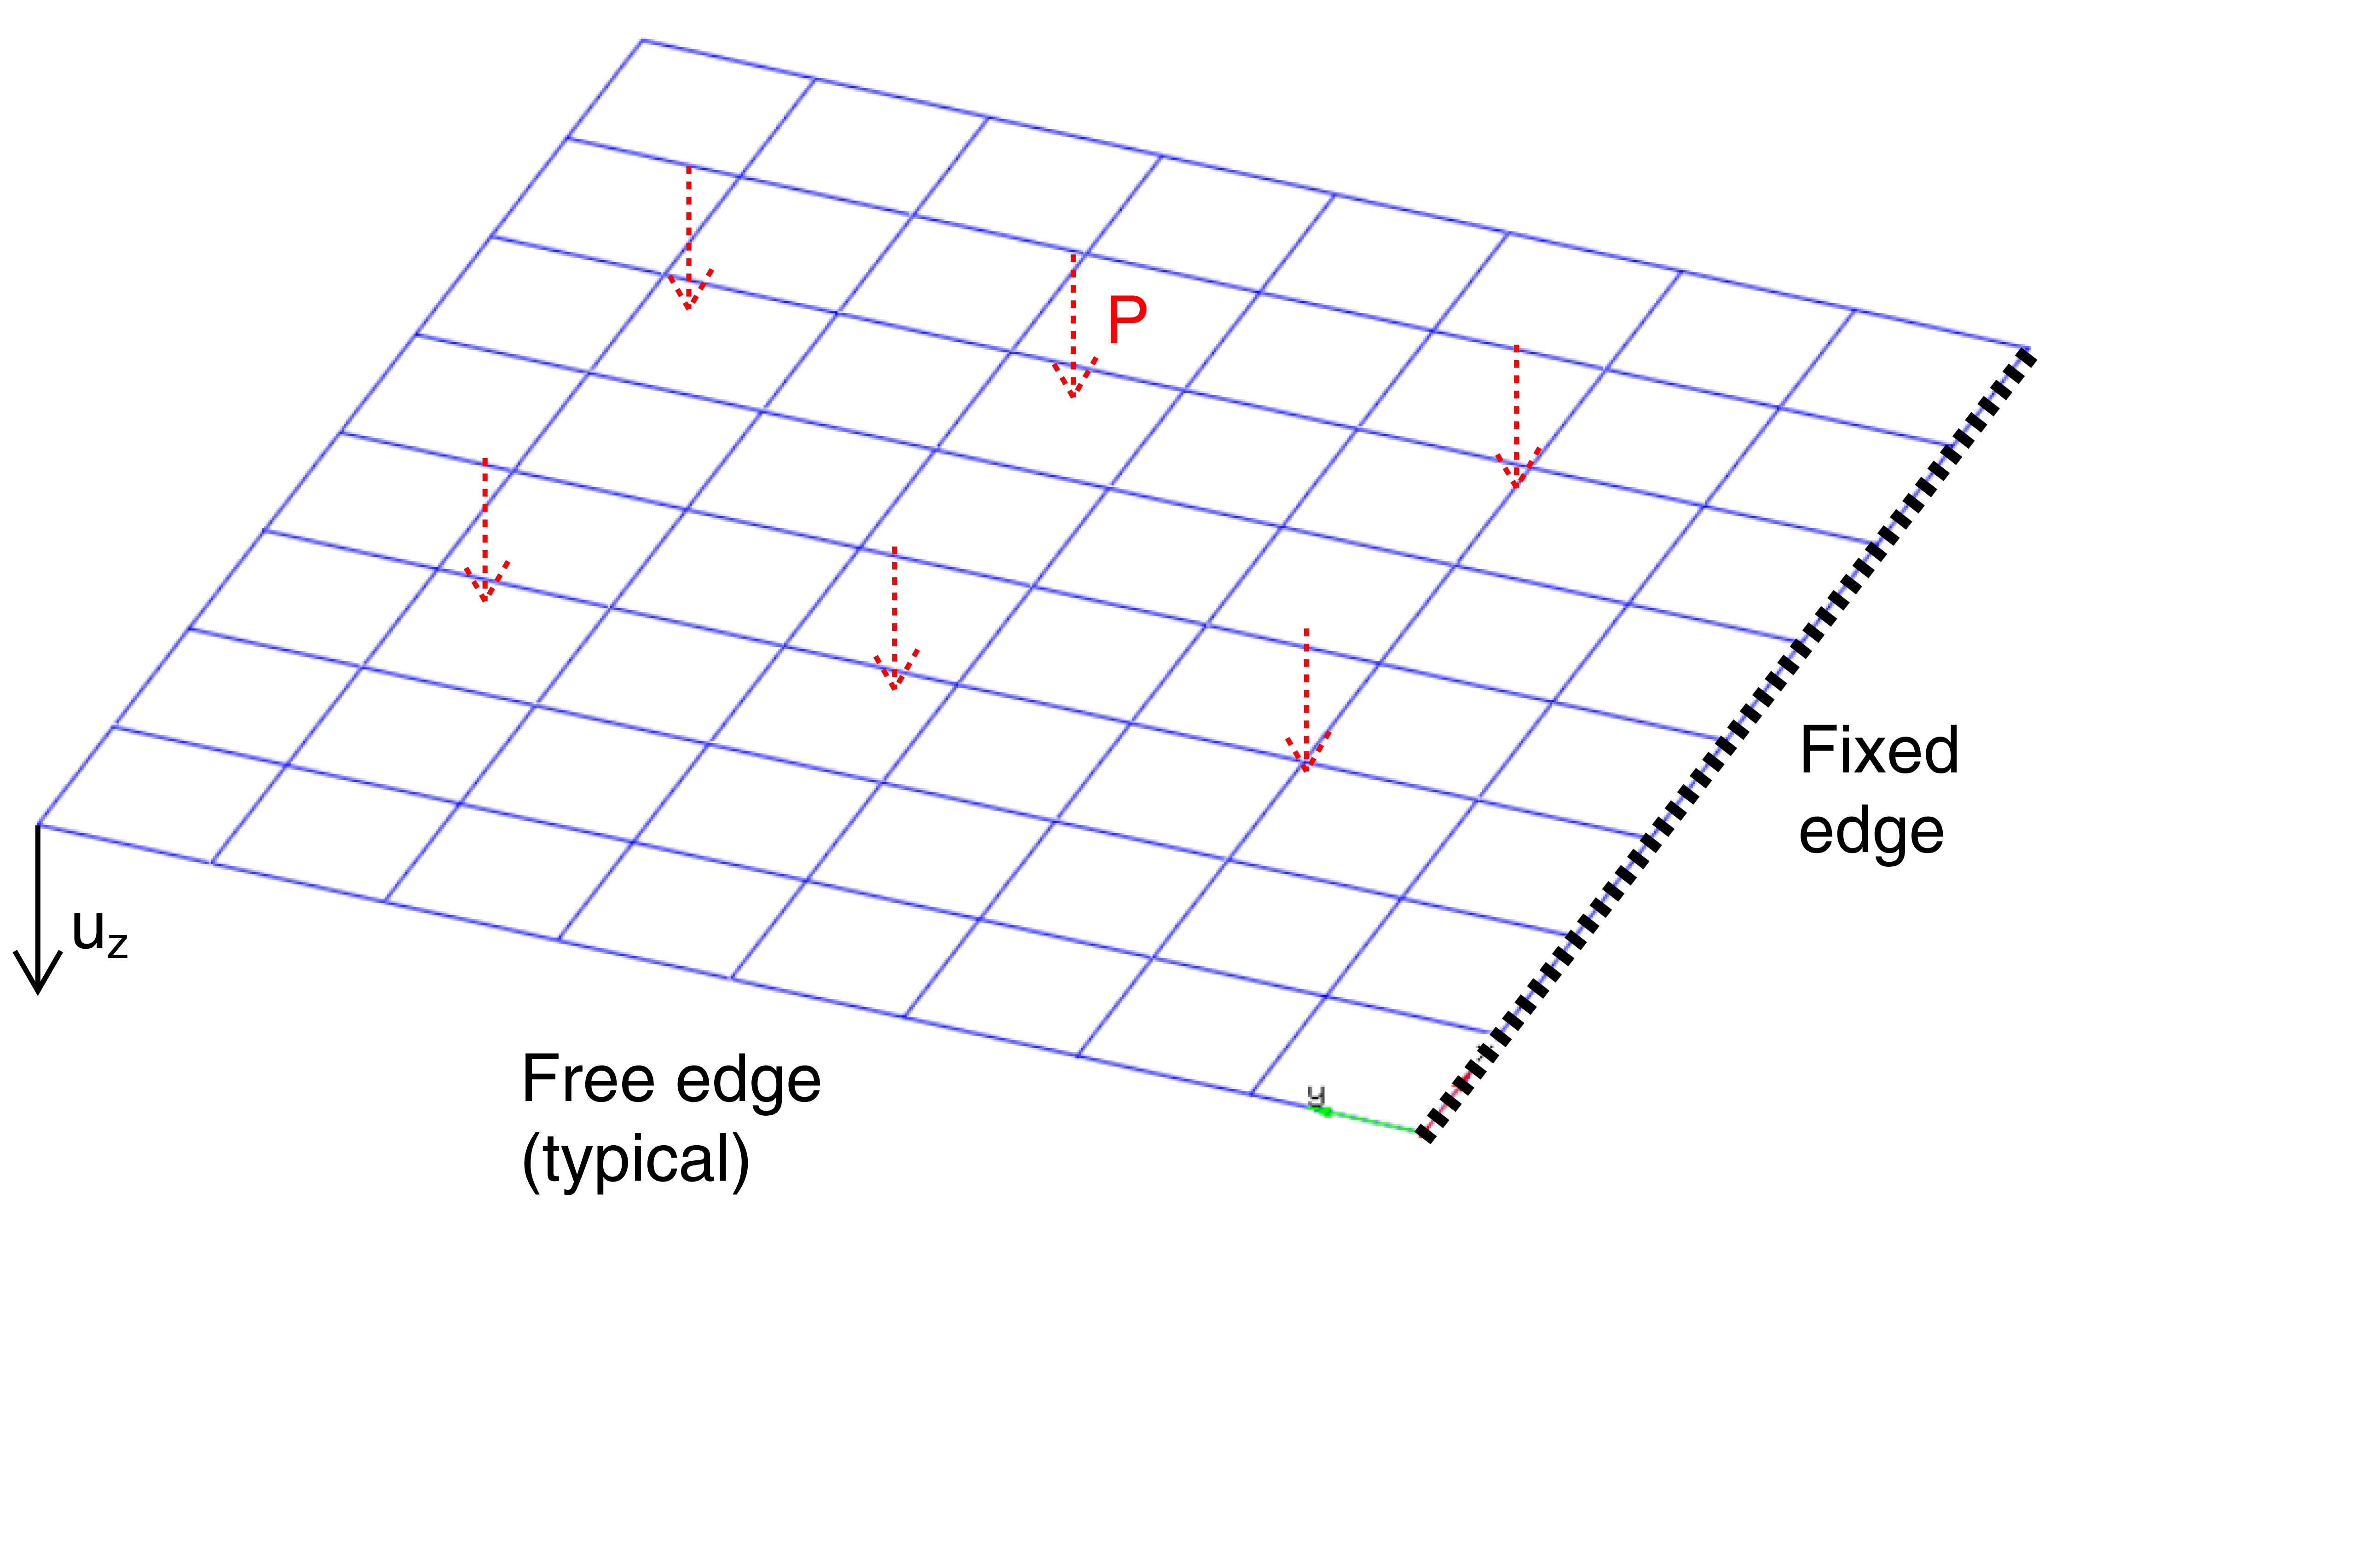
\includegraphics[width=7.3cm]
		{images/quad_bend_problem.png}}
	\subfloat[Vertical displacement over time for Oscillating clamped plate benchmark]
	{\label{ref_label2}
		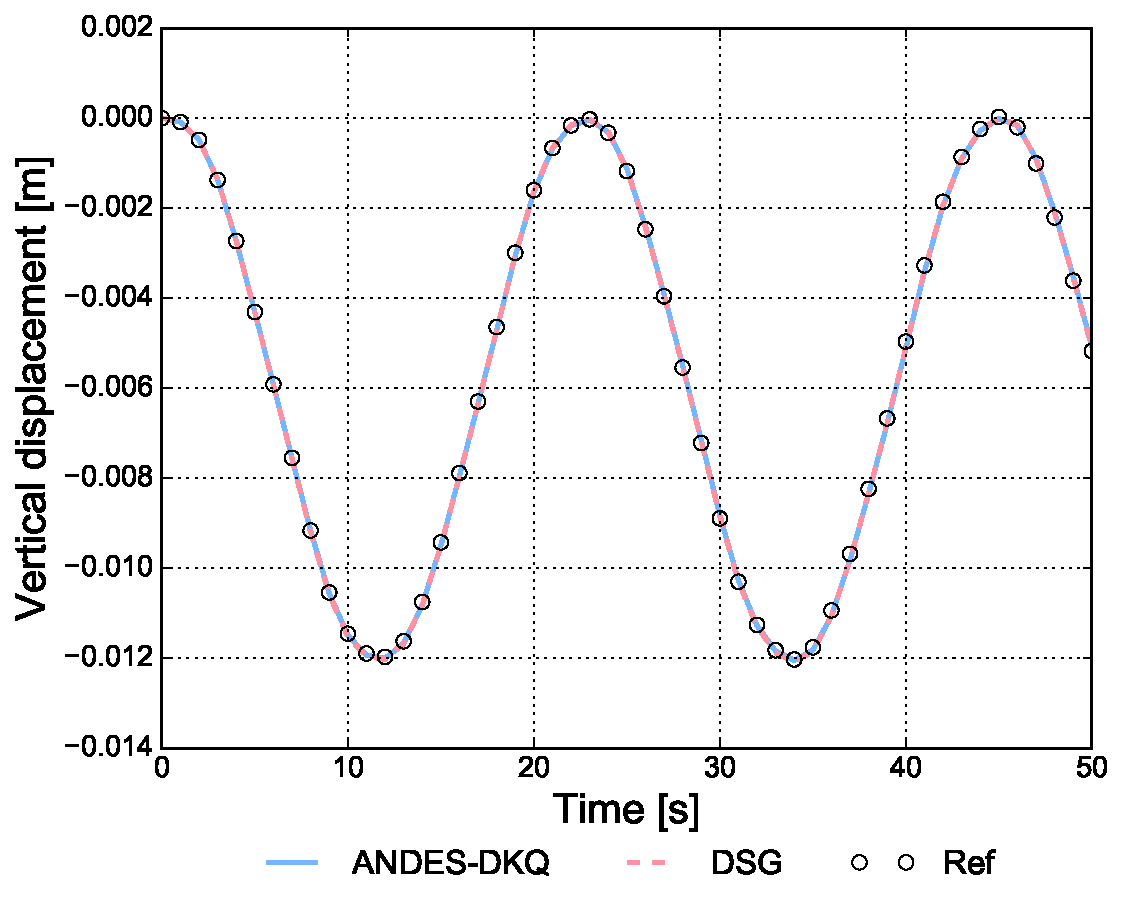
\includegraphics[width=7.3cm]
		{quad_bend_graph.pdf}}
	\caption{\label{Oscillating clamped plate benchmark}Oscillating clamped plate benchmark}
\end{figure}

 The plot of vertical displacement over time demonstrates both elements agree with the reference solution, which is the existing Kratos quadrilateral element. The overall results correctly correspond to structural dynamics theory by oscillating with the base natural frequency about the static displacement of $u_z=-0.006m$.

\section{Quantity recovery benchmarks}

\subsection{Simply supported dome under self weight - done}



Meshes were all roughly 3000 elements.

\begin{figure}[H]
	%\centering
	\subfloat[Circumferential shell force over meridian angle]
	{\label{ref_label1}
		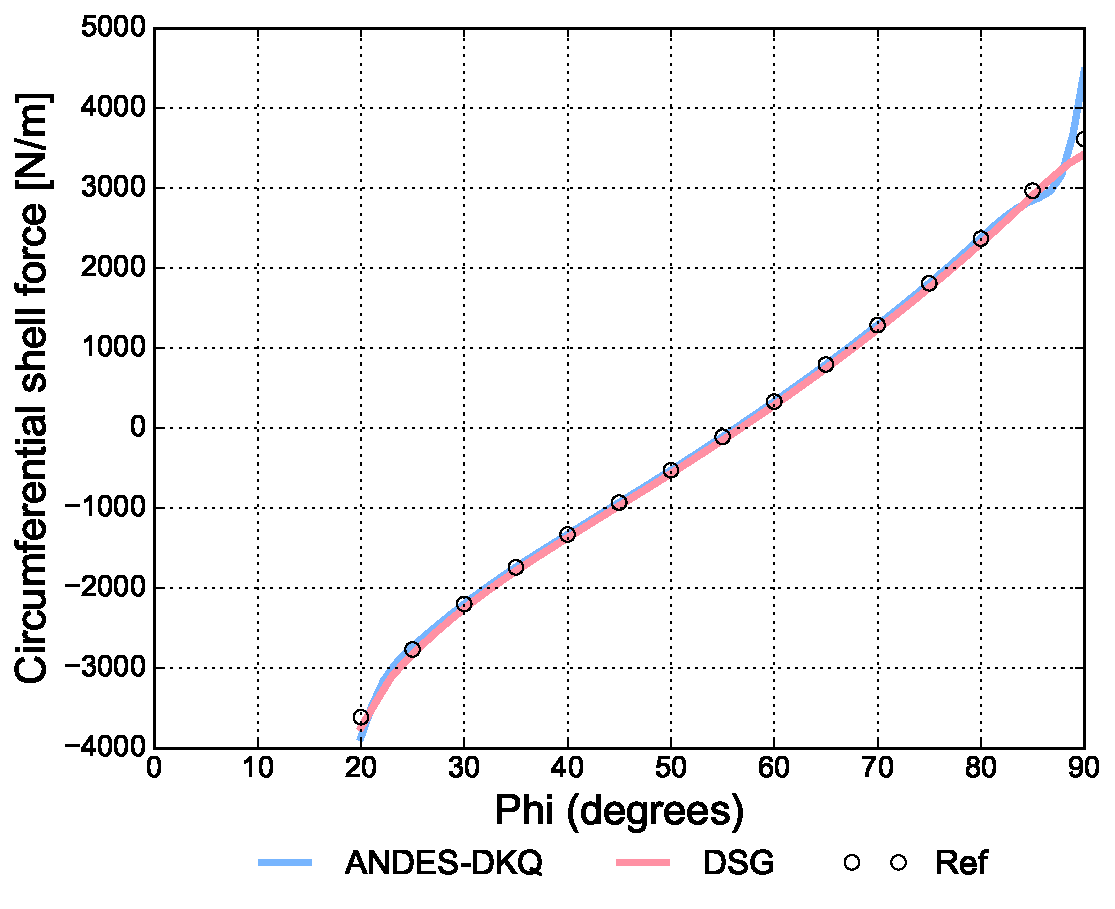
\includegraphics[width=7.3cm]
		{images/Simply_support_dome_n_theta.pdf}}
	\subfloat[Meridional shell force over meridian angle]
	{\label{ref_label2}
		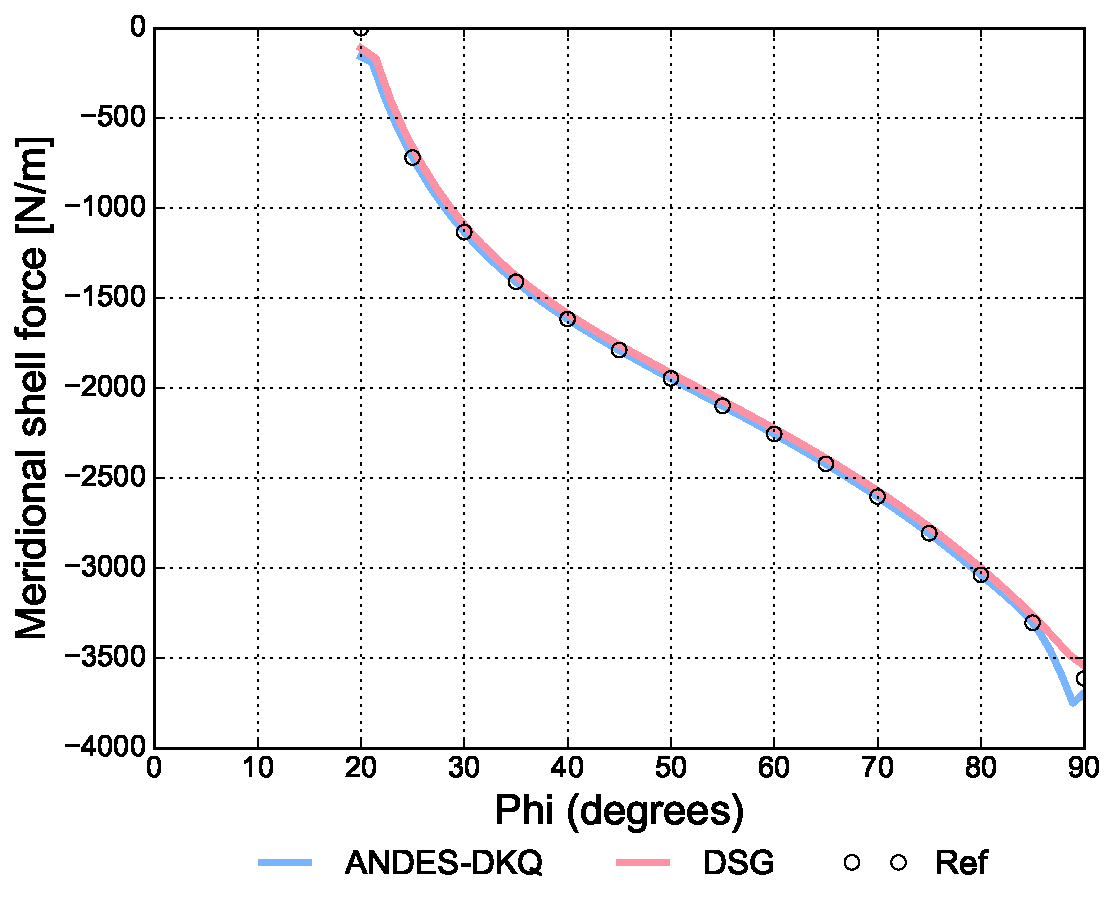
\includegraphics[width=7.3cm]
		{images/Simply_support_dome_n_phi.pdf}}
	\caption{\label{Shell_force_dome_benchmark_shell_force}Shell forces of the simply supported dome benchmark}
\end{figure}

Ref is shell membrane theory!

\begin{figure}[H]
	%\centering
	\subfloat[Mid-plane Von Mises stress over meridian angle]
	{\label{ref_label1}
		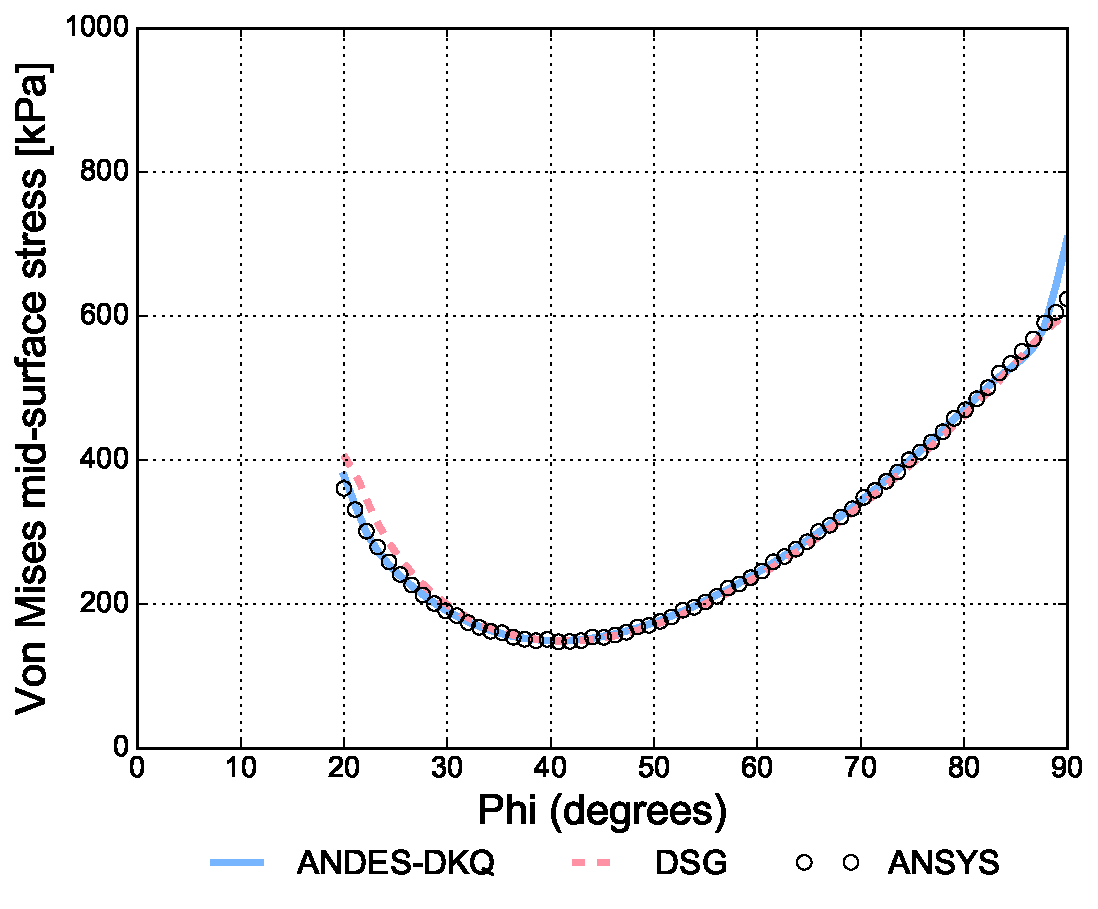
\includegraphics[width=7.3cm]
		{images/Simply_support_dome_von_mises.pdf}}
	\subfloat[Mid-plane Von Mises plot of the reference ANSYS solution]
	{\label{ref_label2}
		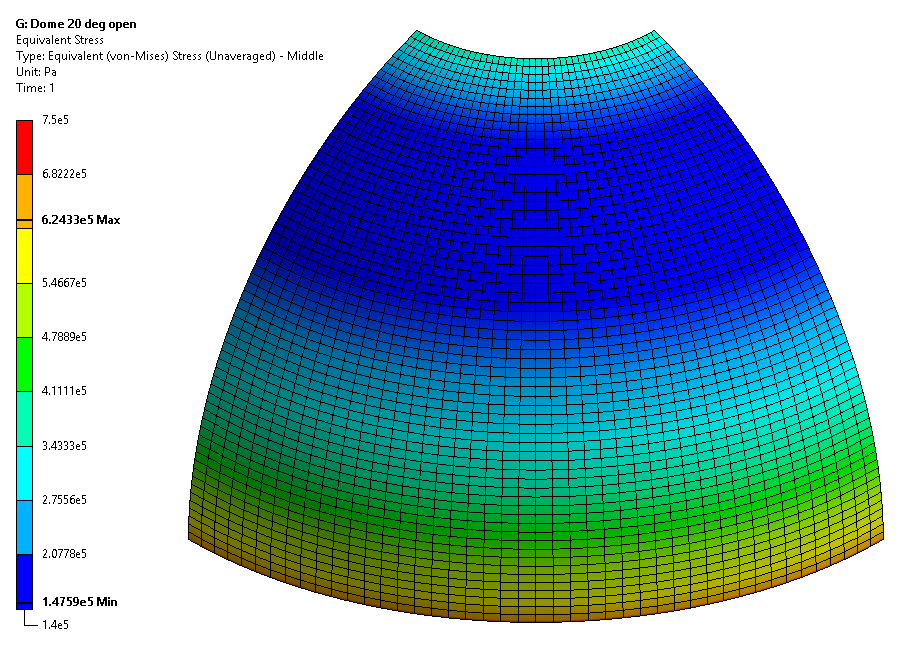
\includegraphics[width=7.3cm]
		{images/simply_support_dome_ansys_vm_plot.png}}
	\caption{\label{Shell_force_dome_benchmark_von_mises}Mid-plane Von Mises stress results of the simply supported dome benchmark}
\end{figure}

\begin{figure}[H]
	%\centering
	\subfloat[Mid-plane Von Mises plot of the ANDES solution]
	{\label{ref_label1}
		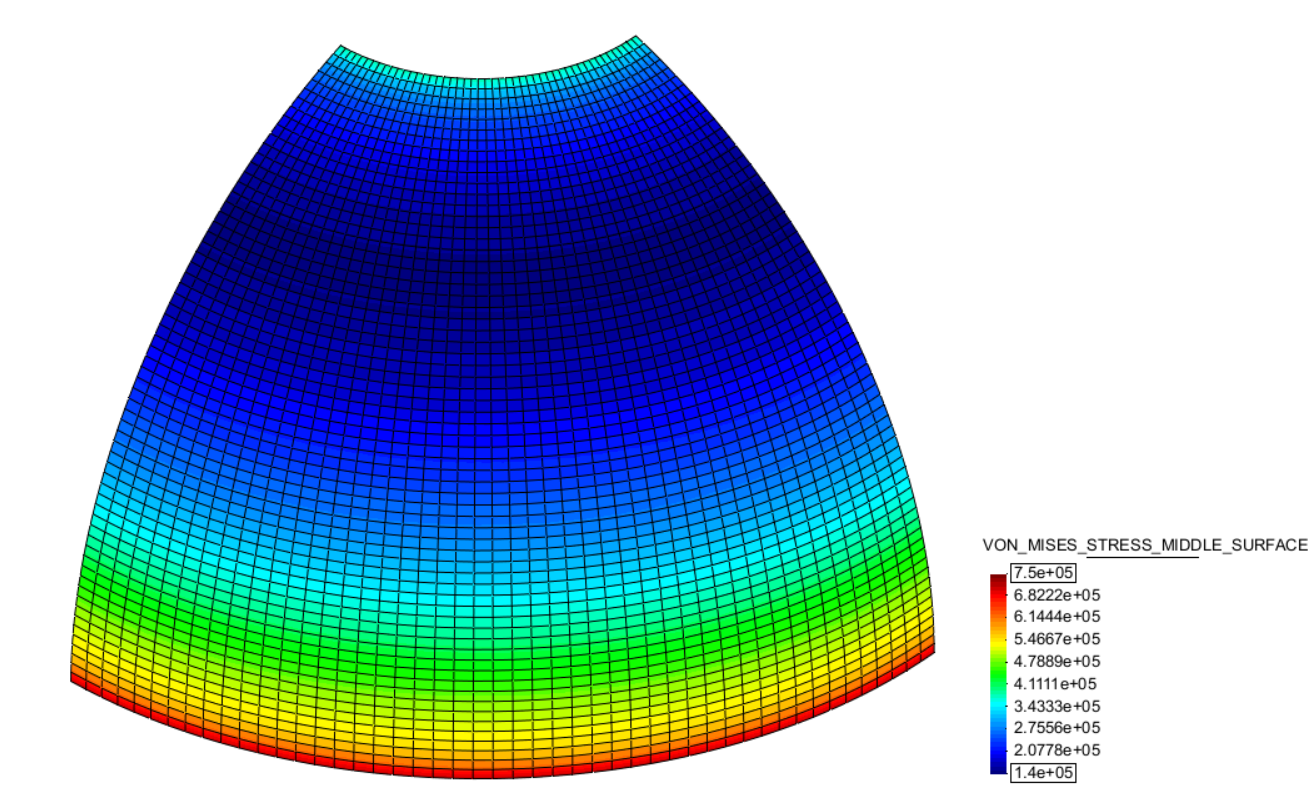
\includegraphics[width=7.3cm]
		{images/simply_support_dome_andes_vm_plot.png}}
	\subfloat[Mid-plane Von Mises plot of the DSG solution]
	{\label{ref_label2}
		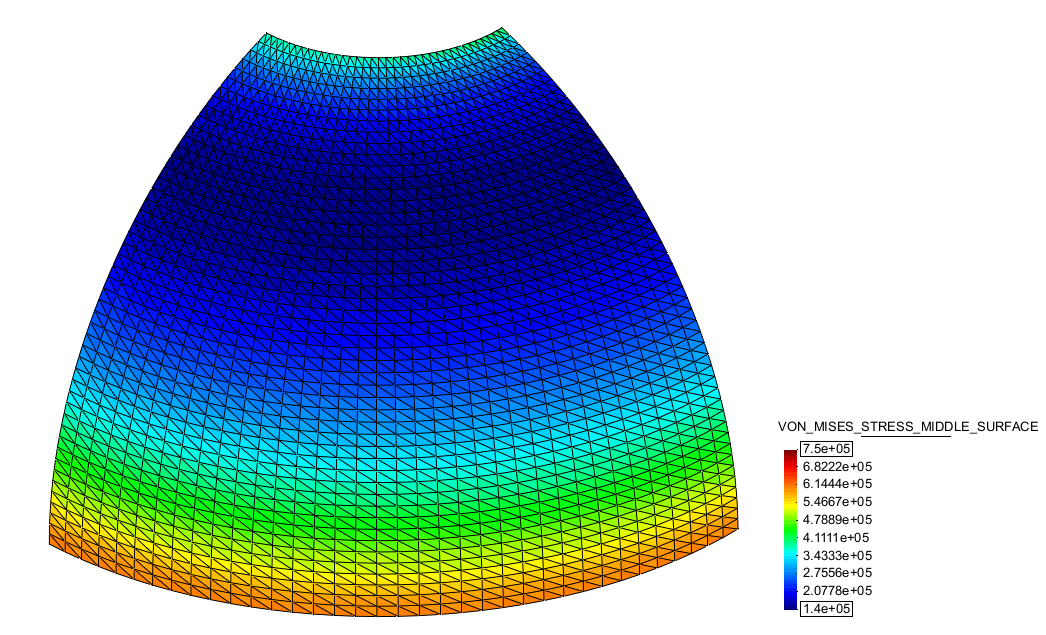
\includegraphics[width=7.3cm]
		{images/simply_support_dome_dsg_vm_plot.png}}
	\caption{\label{Shell_force_dome_benchmark_von_mises_me}Mid-plane Von Mises stress plots of the simply supported dome benchmark}
\end{figure}




limits all set to [1.4e5, 7.5e5] !!!!!!



\subsection{Simply supported plate under uniform pressure - not done}

asdfasdf

\subsection{LEFM SIF recovery - probably skip}

poisson != 0
check strains, forces, moments

\begin{figure}[H]
	%\centering
	\subfloat[LEFM stress concentration factor recovery definition]
	{\label{ref_label1}
		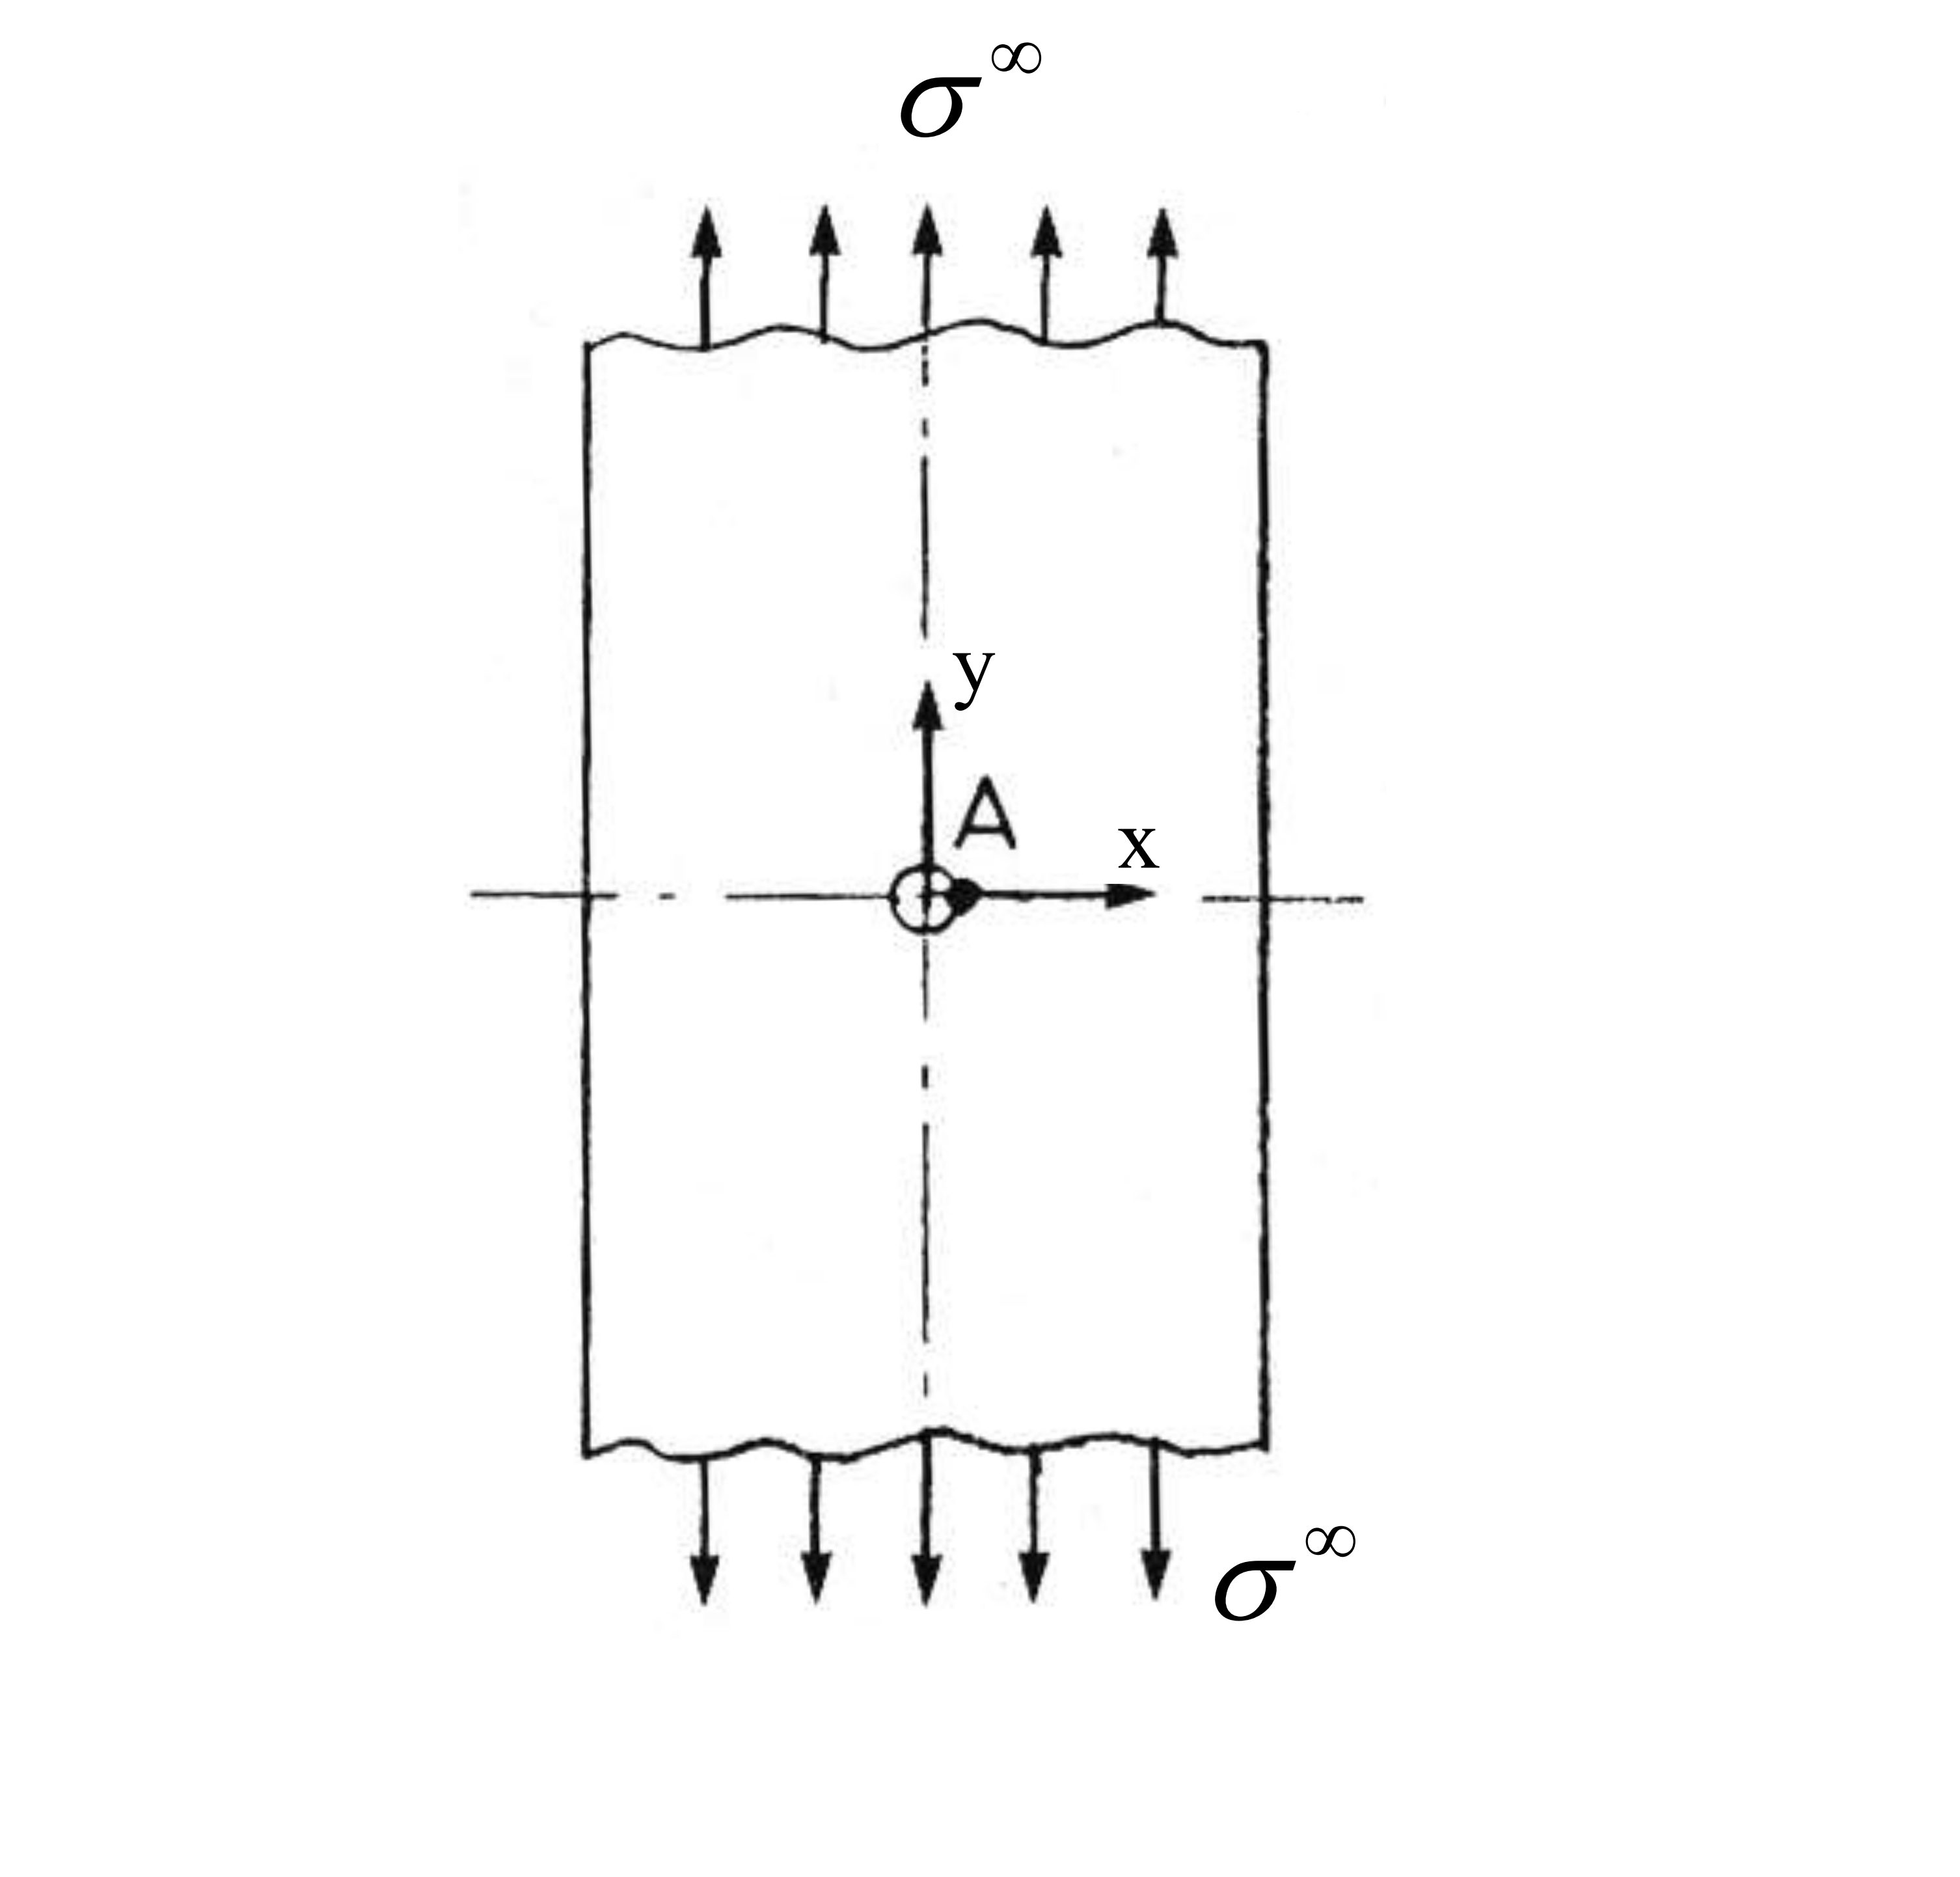
\includegraphics[width=7.3cm]
		{images/plate_with_hole_definition.png}}
	\subfloat[Stress distribution along distance from hole for LEFM stress concentration factor benchmark]
	{\label{ref_label2}
		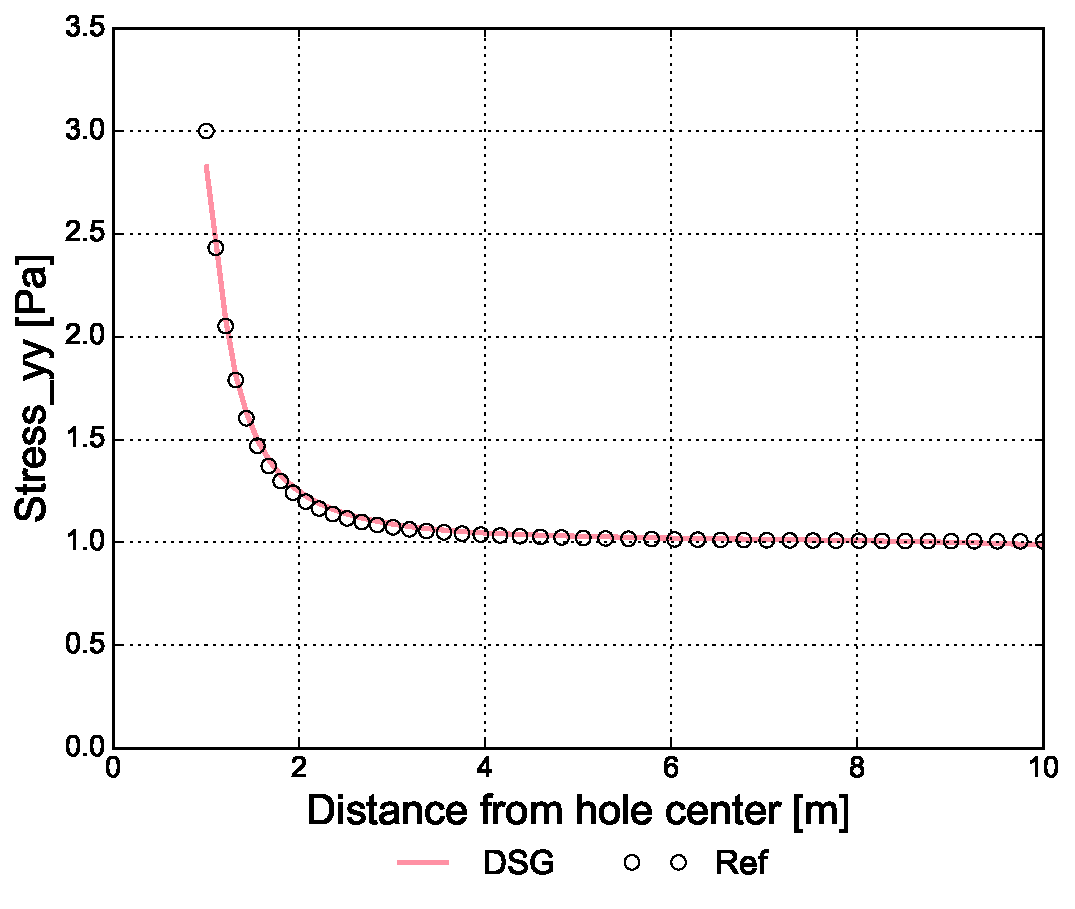
\includegraphics[width=7.3cm]
		{plate_with_hole_results.pdf}}
	\caption{\label{Oscillating clamped plate benchmark}LEFM stress concentration factor benchmark}
\end{figure}

asdf

\section{Composite benchmarks}

asdfadsf

\subsection{Linear static: composite barrel vault - good}

asdfdsf
\begin{figure}[H]
	\subfloat[2 ply cross layup]
{\label{ref_label1}
	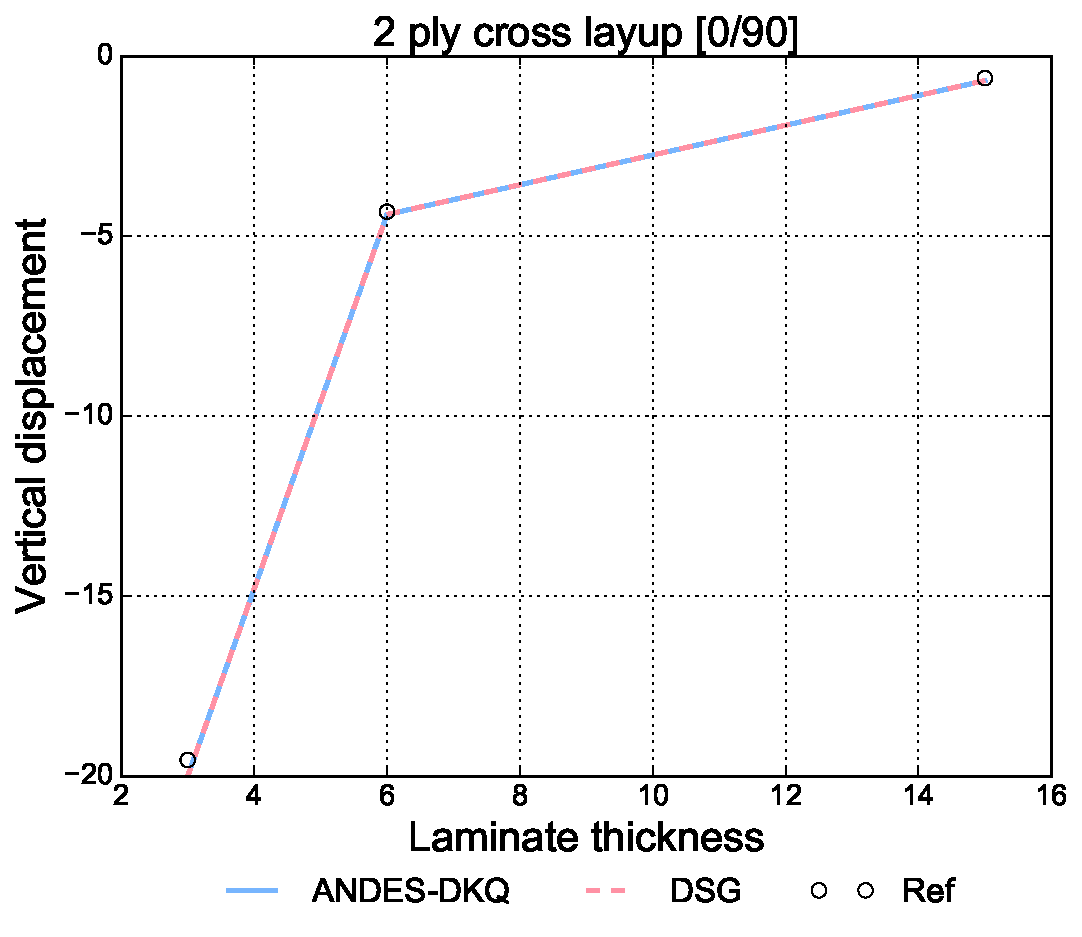
\includegraphics[width=7.3cm]
	{images/cross2ply.pdf}}
\subfloat[10 ply cross layup]
{\label{ref_label2}
	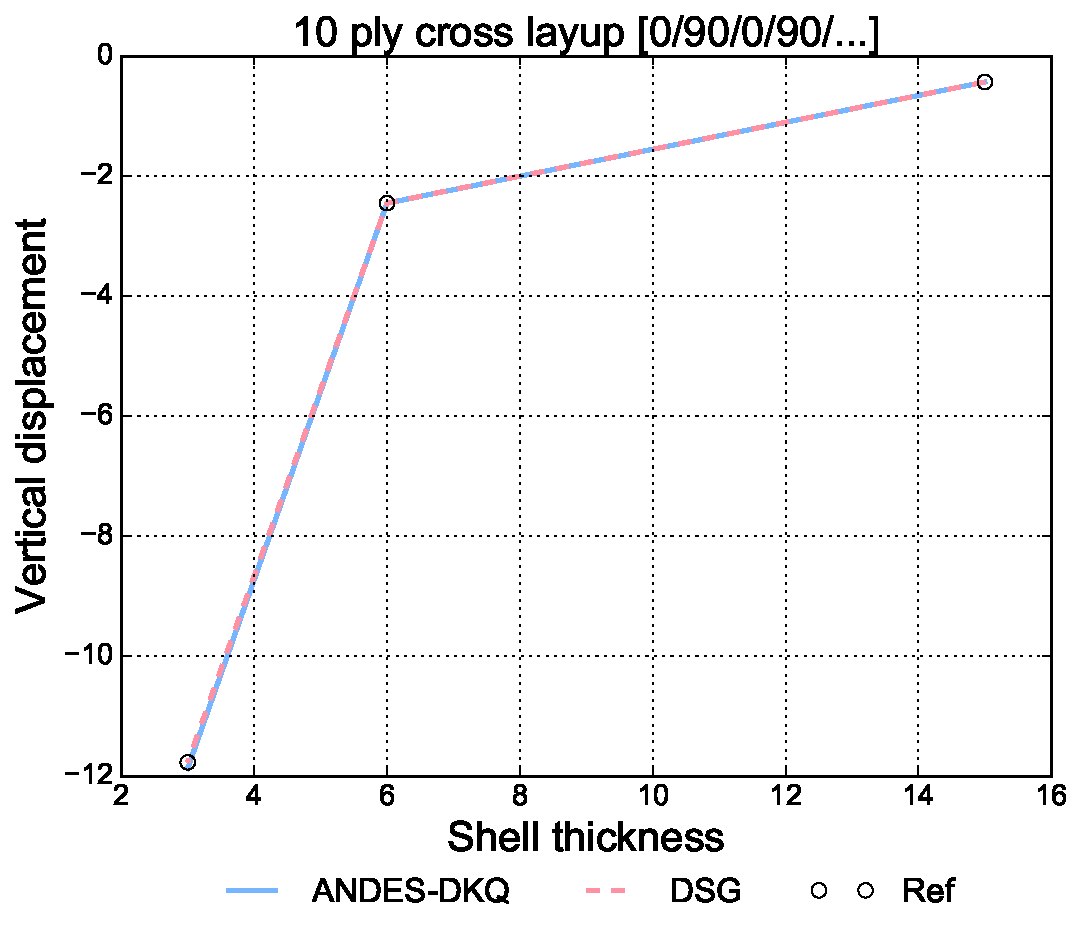
\includegraphics[width=7.3cm]
	{cross10ply.pdf}}
\caption{\label{Composite barrel vault benchmark: cross layup}Composite barrel vault benchmark: cross layup}
\end{figure}

\begin{figure}[H]
	\subfloat[2 ply angle layup]
	{\label{ref_label1}
		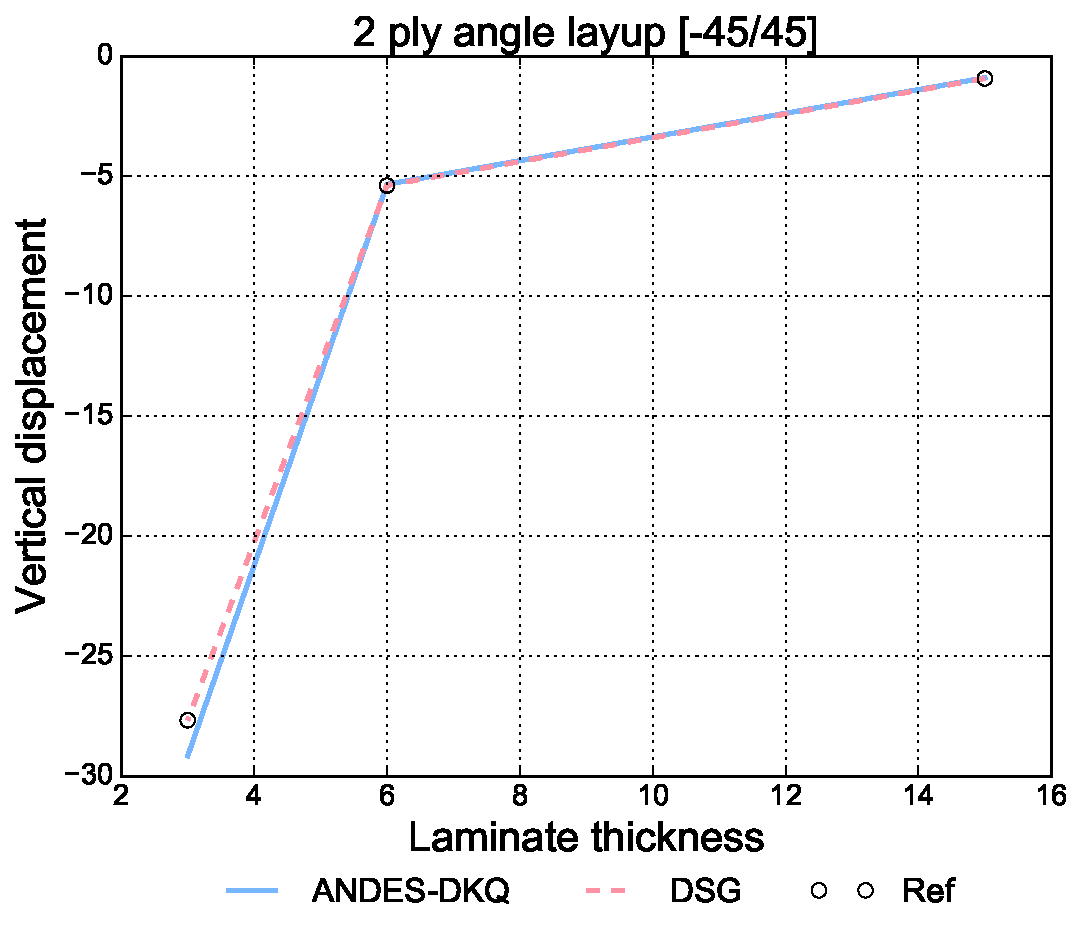
\includegraphics[width=7.3cm]
		{images/angle2ply.pdf}}
	\subfloat[10 ply angle layup]
	{\label{ref_label2}
		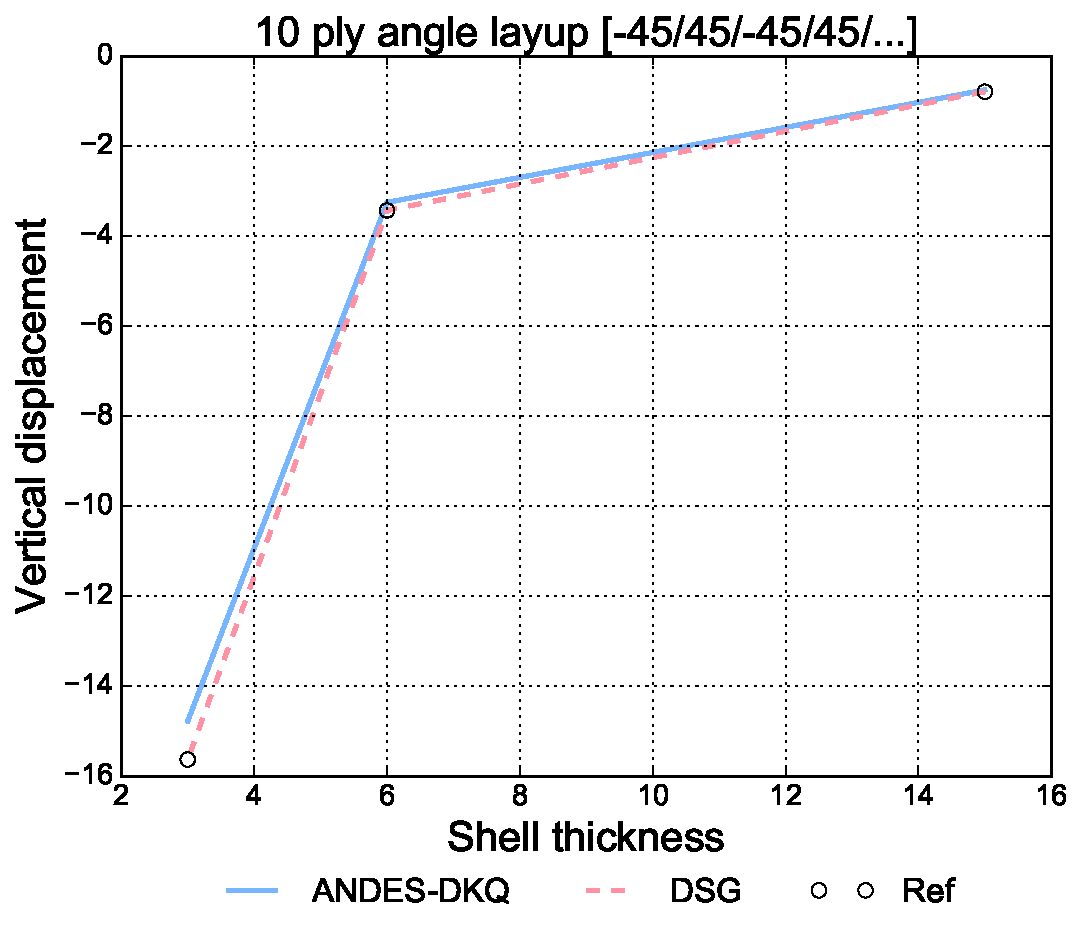
\includegraphics[width=7.3cm]
		{images/angle10ply.pdf}}
	\caption{\label{Composite barrel vault benchmark: angle layup}Composite barrel vault benchmark: angle layup}
\end{figure}

reference solution is \cite{reddy2004mechanics}.

asdfad

\subsection{Linear static: clamped cylinder - good}

asdfdsf

\subsection{Non-linear static: composite hinged cylindrical roof - good}

asdfdsf

\begin{figure}[H]
	%\centering
	\subfloat[Composite hinged cylindrical roof definition \cite{Sze2004}]
	{\label{ref_label1}
		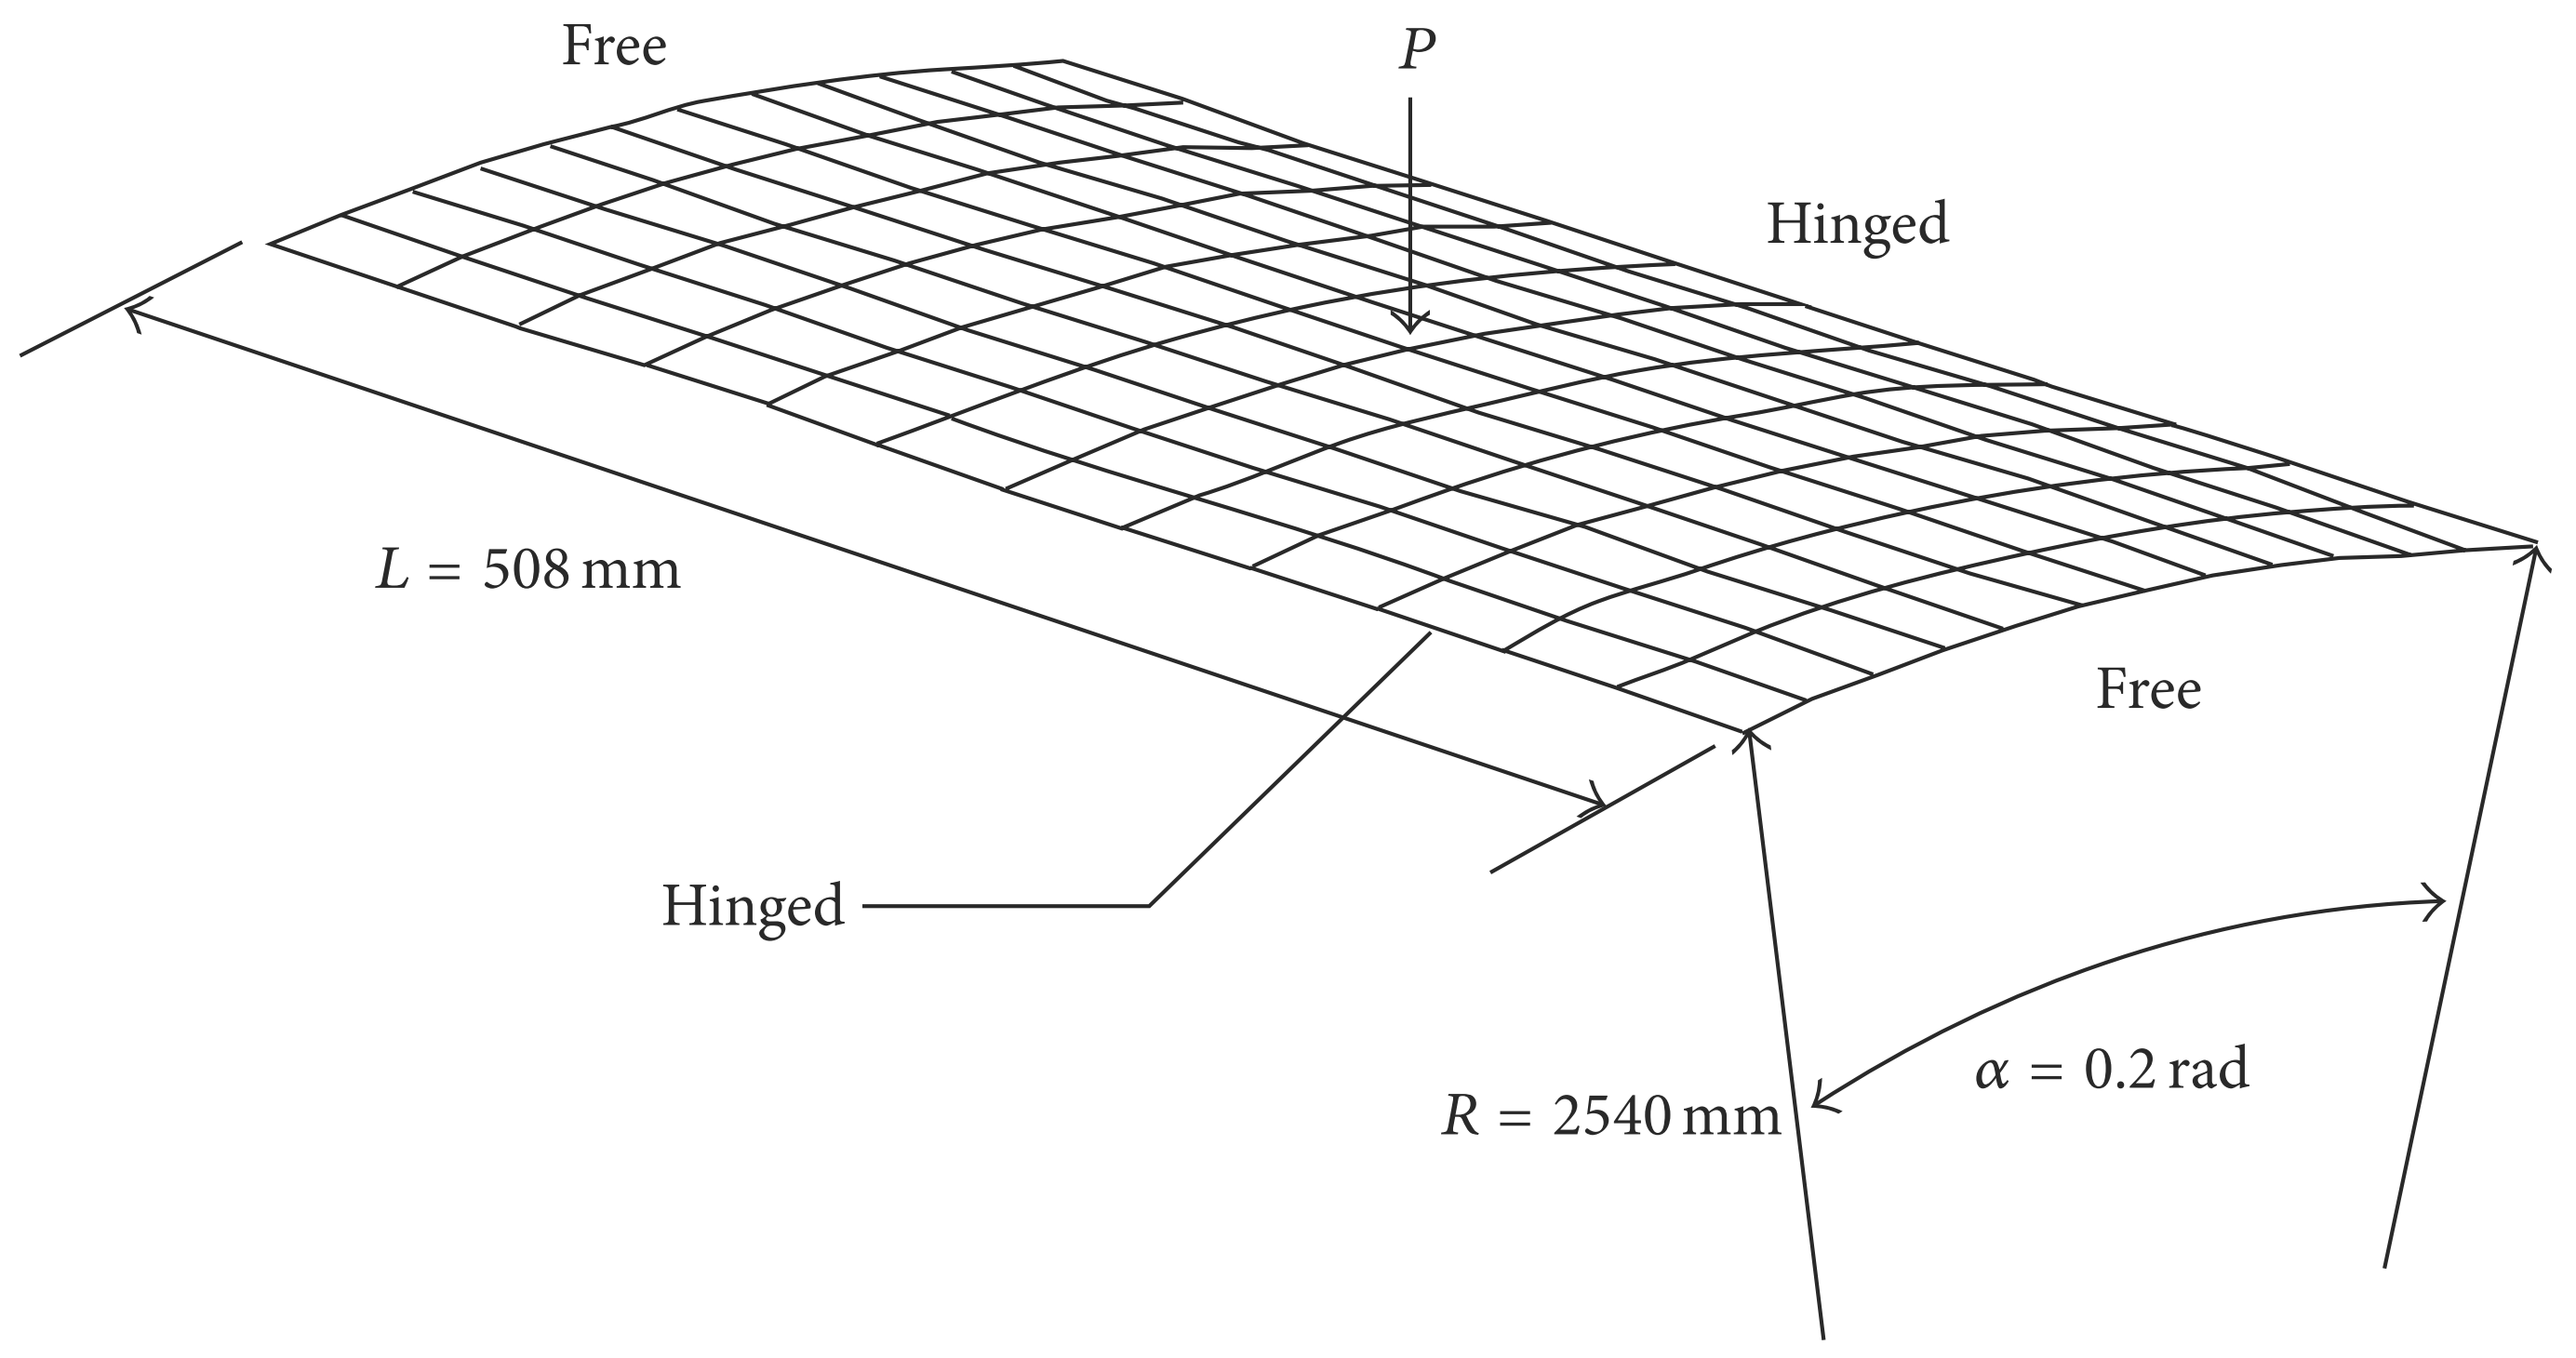
\includegraphics[width=7.3cm]
		{images/hinged_cylindrical_roof.png}}
	\subfloat[Load-displacement curve of composite hinged cylindrical roof]
	{\label{ref_label2}
		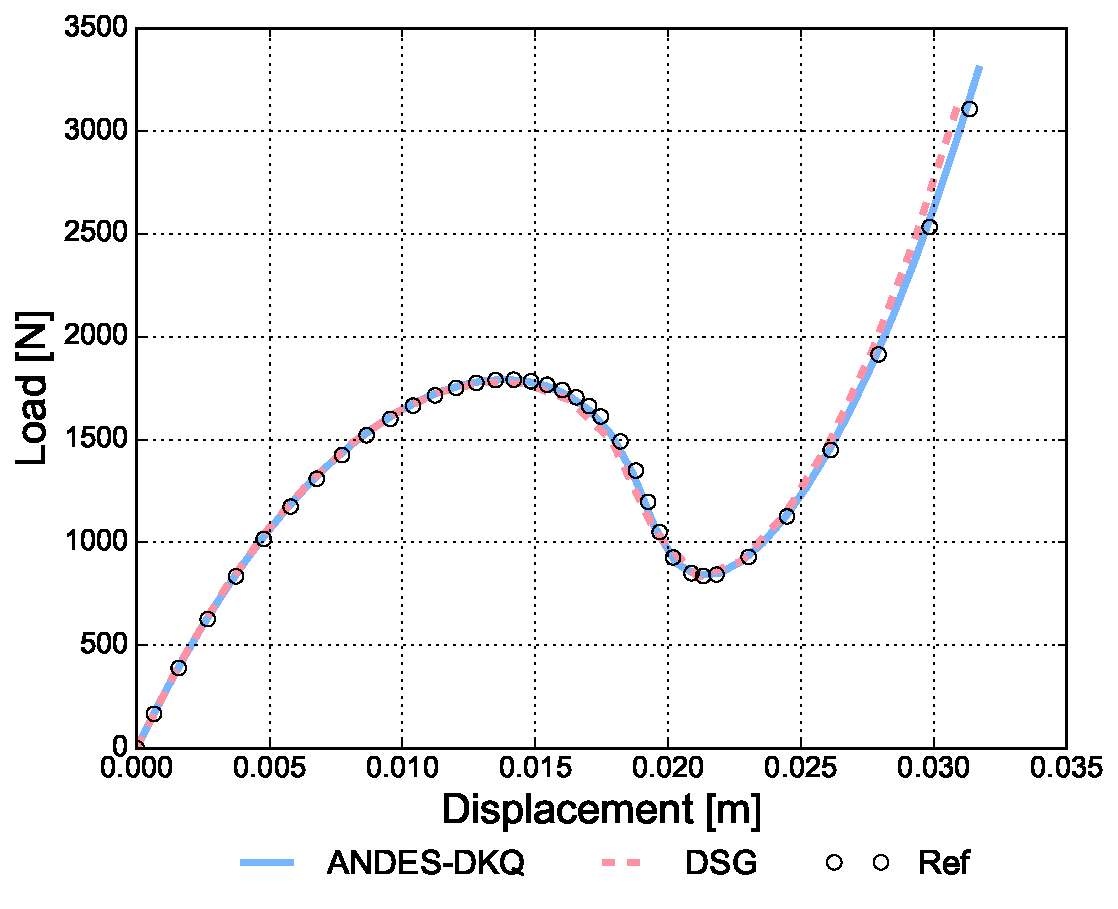
\includegraphics[width=7.3cm]
		{images/Load_displacement_curve_composite_hinged_cylindrical_roof.pdf}}
	\caption{\label{ref_label_overall}Composite hinged cylindrical roof benchmark}
\end{figure}

asdsds

\subsection{Dynamics: shell pendulum - good}

asdfdsf

swinging plate material setup

%	SHELL_ORTHOTROPIC_LAYERS  [4,9] (
%(0.025,0.0,7850,1E+9,1E+9,0.0,1E+9,1E+9,1E+9),
%(0.025,45.0,7850,1E+9,1E+9,0.0,1E+9,1E+9,1E+9),
%(0.025,90.0,7850,1E+9,1E+9,0.0,1E+9,1E+9,1E+9),
%(0.025,135.0,7850,1E+9,1E+9,0.0,1E+9,1E+9,1E+9)
%)

\begin{figure}[H]
	%\centering
	\subfloat[Vertical displacement over time for composite shell pendulum benchmark]
	{\label{ref_label2}
		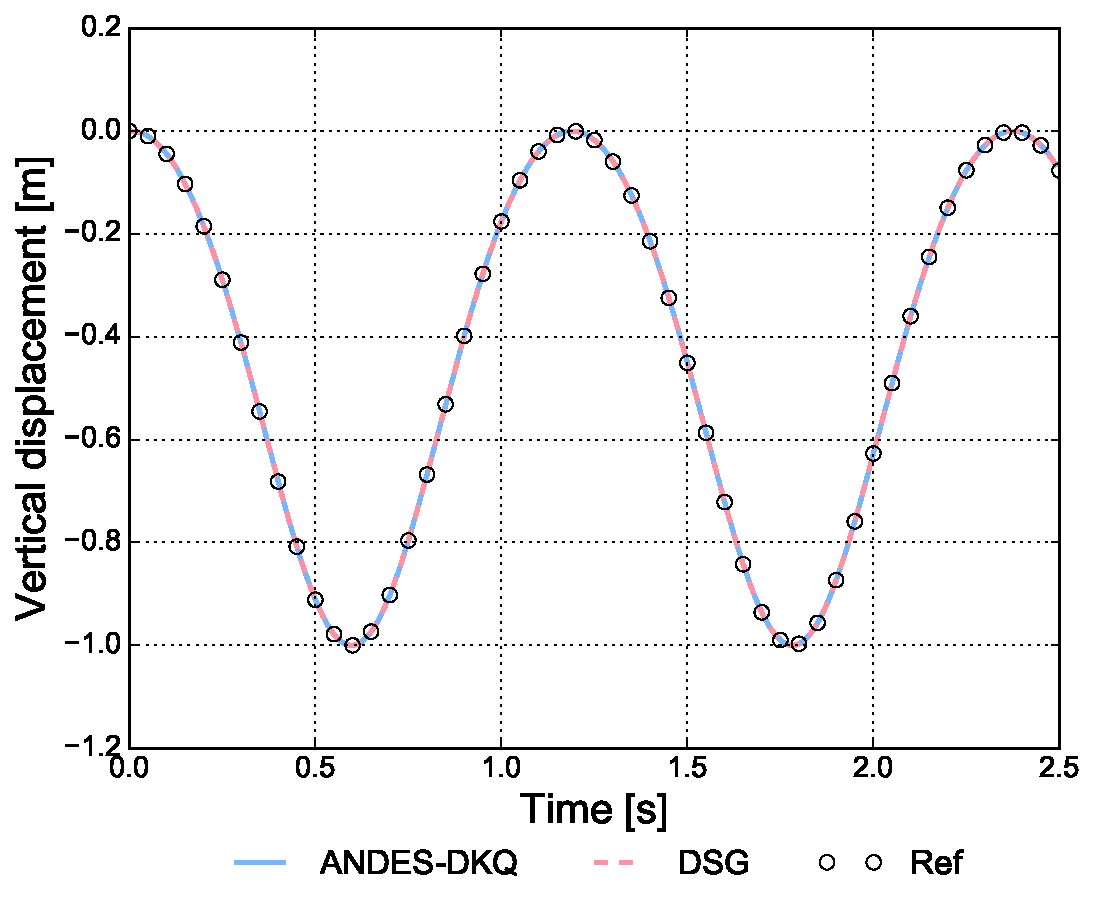
\includegraphics[width=7.3cm]
		{images/swinging_plate_composite_graph.pdf}}
	\subfloat[Vertical displacement over time for composite oscillating clamped plate benchmark]
	{\label{ref_label2}
		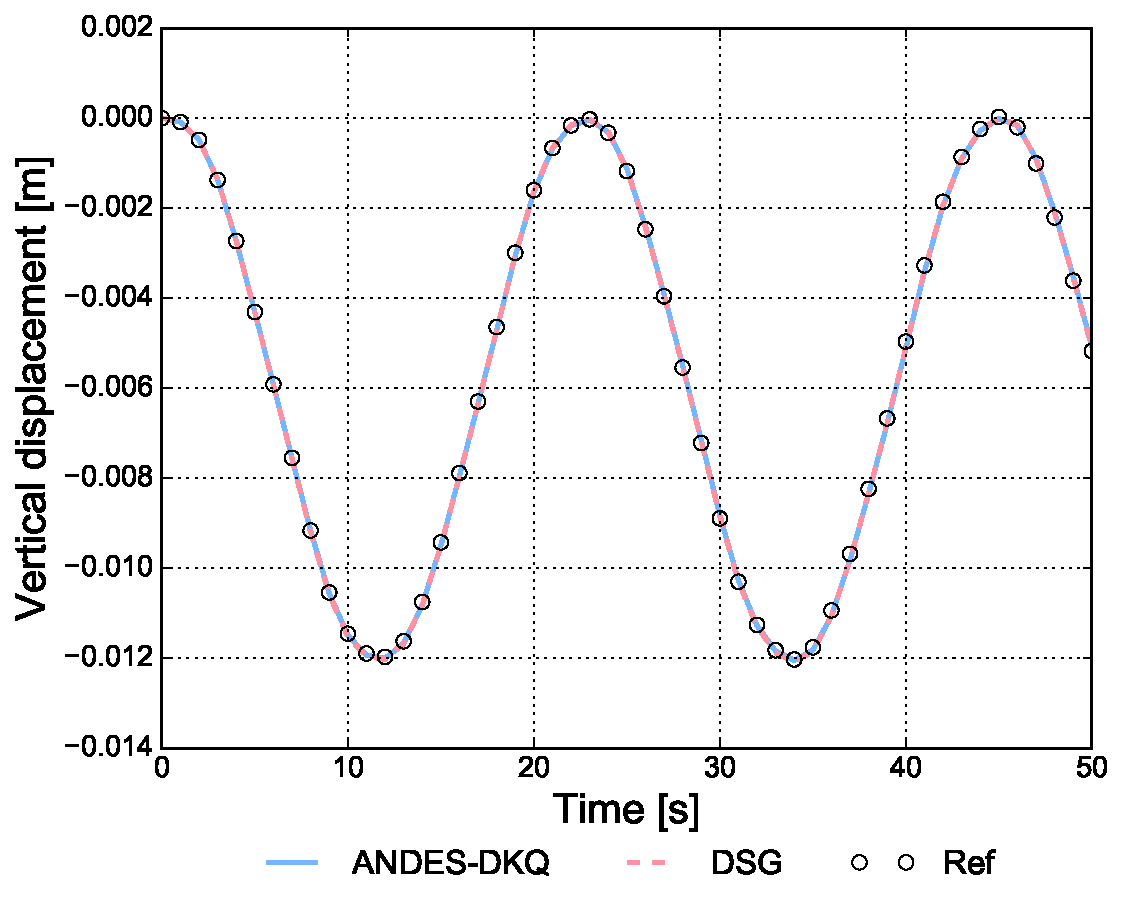
\includegraphics[width=7.3cm]
		{images/quad_bend_composite_graph.pdf}}
	\caption{\label{Composite dynamic benchmarks}Composite dynamic benchmarks}
\end{figure}

oscillating plate setup

%	SHELL_ORTHOTROPIC_LAYERS  [4,9] (
%(0.250000E-001,0.0,7850,1.00000E+06,1.00000E+06,0.0,0.50000E+06,0.50000E+06,0.50000E+06),
%(0.250000E-001,45.0,7850,1.00000E+06,1.00000E+06,0.0,0.50000E+06,0.50000E+06,0.50000E+06),
%(0.250000E-001,90.0,7850,1.00000E+06,1.00000E+06,0.0,0.50000E+06,0.50000E+06,0.50000E+06),
%(0.250000E-001,135.0,7850,1.00000E+06,1.00000E+06,0.0,0.50000E+06,0.50000E+06,0.50000E+06)
%)

replace with composite results!!!!

\subsection{Stress recovery: tensile test - good}

asdfdsf

\subsection{Stress recovery: simply supported plate under uniform pressure - not done}

asdfdsf